
The development process outline was inspired by the
twelve key-principles of user-centered system design
listed earlier, especially the following ones:
\textit{user focus},
\textit{active user involvement},
\textit{evolutionary systems development},
\textit{simple design representations},
and
\textit{prototyping}.
%The overall process took inspiration from agile software development with a
%touch of 'design-school'. \todo{Fix this section.}

%Since the resulting application should be something that could potentially
%benefit the team, with the users

\begin{figure}[h!]
  \centering
  \includegraphics{figures/method.pdf}
  \caption{Concept, development, testing and improvement cycle.}
\end{figure}

%The user focus should be established by the initial interviews. By interviewing
%for actual pain-points, in this case from managers, finding a
%Using the initial interviews, the goal was to figure out what kind of
%project could be constructed

\section{Brainstorming-sessions and interviews}{\label{label_sectionIdeas}

%\todo{ Ta bort den del som handlar om vad du initialt tänkte men som inte blev
%av. Förtydliga att fokus är på webbaserad testning men att för att kunna testa
%det på något relevant har du, genom intervjuer, hittat ett område (workload,
%hours, etc) som du använder för att exemplifiera ditt webbaserade testsystem.}
%
%\todo{ Här kanske också är ett bra ställe att presentera målgrupp (primary
%users...) om det ej är gjort tidigare. }

One of the initial ideas, what later became the employee-hours test-task, came
from a comment during a general discussion on what could be an interesting
result from the project for the company. A manager expressed that they would
like better tooling for working out if any of their co-workers has to much work
assigned to them. Stating that having better access to this information would
make it easier to smooth out work-spikes, and distribute work more evenly,
benefiting the team overall, and in extension, the company.

Discussing the possibility for managerial or more general tooling further, it
became apparent that any such application, in addition to being easily
accessible internally, need to be available for employees in off-site work
situations. Given this, it was determined that a web- or networked-based
solution would be the best fit for any such application or tooling-extension.

Bringing these ideas back to the supervisor in order to determine possible
initial directions and academic application, the issue of design and
usability-testing came up. This was extra important since the
chosen design and development process was both iterative and user-centric, two
methodologies that benefit from having frequent and high-volume tests done in
order to gather feedback and data to feed back into the process.

While discussing how this type of testing could be performed and scaled towards
a large company while only having limited time and man-power, the connectivity
requirement came up once again. Since theoretically, some of the end-users
could be off-site, and we would sill like to have them in the available testing
pool, the same access criteria applies to the tests, in short, the
testing-platform should also be web-based and accessible through the network.

Weighing the options at the time, the testing-platform was chosen as the main
focus of the project given it had the possibility to provide interesting
feedback on the viability of distributed usability-tests in game-development,
with both players or hired testers. Additionally, instead of scrapping the
tools-angle, it was retrofitted to become the basis for the test-task running
on the platform. This was done in order to give the tests a grounding in
real-life and if possible, gather some data that could be used as guidance
should said tooling be developed in the future. More in-depth information about
the test-tasks can be found under section \ref{label_basis_purpose} at page
\pageref{label_basis_purpose}.

With this starting point established, in-person interviews were conducted
in order to figure additional tooling that could provide benefit if developed.
The interviews were conducted with four managers from Massive, and focused on
what, if anything, they felt was missing from their day-to-day digital
managerial-toolbox, producing the following wish-list, the initial
suggestion included:


  \newcommand{\ideaOne}{%
    An easy way to see if a co-worker is assigned more work than they have
    available hours.%
  }

  \newcommand{\ideaTwo}{%
    Calendar overview where it is possible to determine if there are
    hot-spots where lots of results need to be produced at the same
    time.%
  }

  \newcommand{\ideaThree}{%
    A concise way to identify if there are critical tasks that, if
    delayed, would delay other tasks that depend on it.%
  }

  \newcommand{\ideaFour}{%
    The possibility to identify a group or teams strengths and assign
    task types accordingly.%
  }

  \begin{itemize}
    \item{\ideaOne\label{label_ideas}}
    \item{\ideaTwo}
    \item{\ideaThree}
    \item{\ideaFour}
  \end{itemize}

\section{Design sketches}

%  \todo{Bra att du knyter an till detta. Ge gärna något konkret exempel på hur
%    detta påverkat din design.}
%
%  \todo{
%    Du behöver också förklara grunden i designen,
%    varför är det detta innehåll? Det är ju inte alls säkert att den vyn som
%    heter View-data passar det som skall presenteras för respektive område och
%    att en "view-additional" behövs. Fanns någon tanke här eller är det mest
%    ett ad-hoc-förslag?
%  }
%
%  \todo{
%    Knappt att du skall kalla det lofi-prototyp då det ej är har någon
%    interaktivitet. Skiss är kanske bättre ord.%
%  }
%

	The overarching goal of the design sketches was to create simple yet
	representative paper-mock-ups of possible platform-interfaces. These
	representations  could then be quickly evaluated through a few in-person
	interviews, and the winning concept would then be implemented as a basic
	interactive web-application for further analysis and design-iteration.

	For this purpose, there were two books that served as inspiration, namely;
	\citeauthor{citeDonMakeMeThink}s
	\citetitle{citeDonMakeMeThink}\cite{citeDonMakeMeThink} and Donald Normans,
	oft-cited design classic,
	\citetitle{citeTheDesignOfEverydayThings}\cite{citeTheDesignOfEverydayThings}.

	\subsection{Sketch elements, affordances and signifiers}

	Searching for ideas and pointers for the general design, a simple but
	actionable idea was lifted from Krug, ''Break up pages into clearly defined
	areas'', witch in this particular example manifests as the boxy design with
	clearly defined borders and wide gutters between all the elements.

  As for navigation, it was known that there would be more than one tests-task
  running on the platform, therefore there needs to exist a way for the
  participants to select which test to run. Here the most obvious solution was
  chosen, four buttons, one for each task-type, that when clicked would display
  the chosen test-task. This solves the task-selection problem, but introduces
  another design-issue instead. Since the goal is to keep initial sketch as
  simple as possible, the same graphical element is used for all the different
  interface elements, making it possible for participants to confuse what part
  of the interface that are buttons or not.

	Looking to Norman for a solution, there are two terms that come to mind,
	\textit{affordace} and \textit{signifiers}. In the context of the book,
	affordaces describe the possible interactions between people and the
	environment they are in, or more precisely in this example, what type of
	actions can the participants perform while visiting the web-application. As
	for the second term, signifies, Norman describes them as design-elements that
	signals things, in particular what actions are possible, and how they should
	be done.

  In regards to affordances, there is not much that can be done in this
  case. Since the testing-platform is web-based, it will automatically inherit
  the affordances one would typically associated with a web page or web
  application. Namely, a web-page will most likely have some information
  displayed as text that can be read, and in most cases there will also be some
  buttons or links that when clicked, either takes us somewhere else or change
  the currently displayed information.

	Looking at the second option, signifiers, they provides more possibilities
	for active design-decisions. Given that the main purpose of a signifier is to
	signal what action can be performed, the signifier attached to the buttons
	need to signal that the buttons can be clicked. Going back to Krug, there is
	a second idea he presents in the book that dovetails nicely with Normans
	signifiers discussion, namely ''Make it obvious what's clickable''. Here he
	recommends that by simply having a distinct color for clickable elements and
	never using that particular color on non-clickable elements should get you
	most of the way there.

	In summary, the different areas and elements of the interface should be given
	a distinct border, and be separated by a gutter in order for them to be
	easily differentiated. As for buttons, their design should include clear
	signifiers about their 'clickability', this is achieved by following Krugs
	advice and make each of the them share the same distinct set of restricted
	colors that are not repeated anywhere else in the interface.

	\newpage
	\subsection{Layout and final design-sketches}

	With the general design characteristics of the elements figured out, the
	amount and type of elements making up the sketch needs to be defined. We know
	we have four button elements that need to have their corresponding task-data
	displayed somewhere when clicked. In order to facilitate the task-data
	viewing a large portion of the interface will be assigned to the
	\textit{View-Data} element.

	While discussing possible task-designs, there were examples that would
	benefit for secondary controls, such as date-ranges and personnel-selectors,
	which, if needed would be placed in the \textit{View-Additional} element.

	With all the components defined we can apply some different layouts in order
	to create a few different versions, presented below, that can then be
	evaluate by the interviewees.

	\begin{figure}[h!]
		\center
		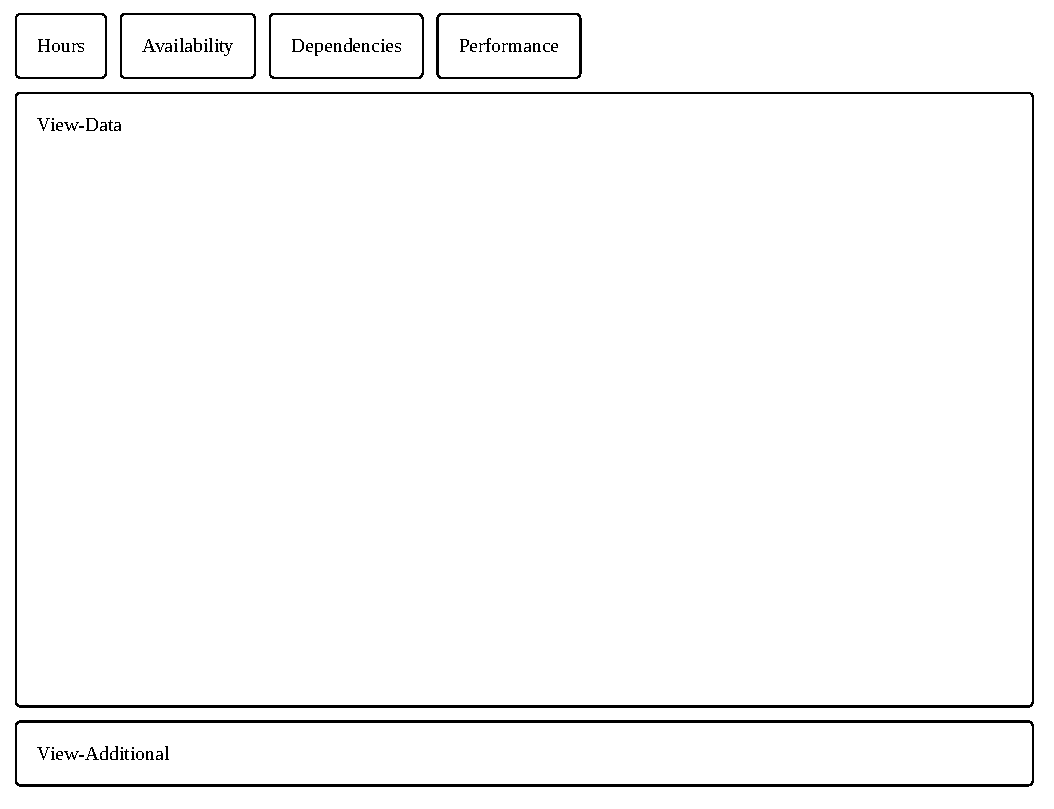
\includegraphics[valign=t,trim={.15cm .10cm .35cm .22cm},clip,width=.49\linewidth]{ui11.pdf}
		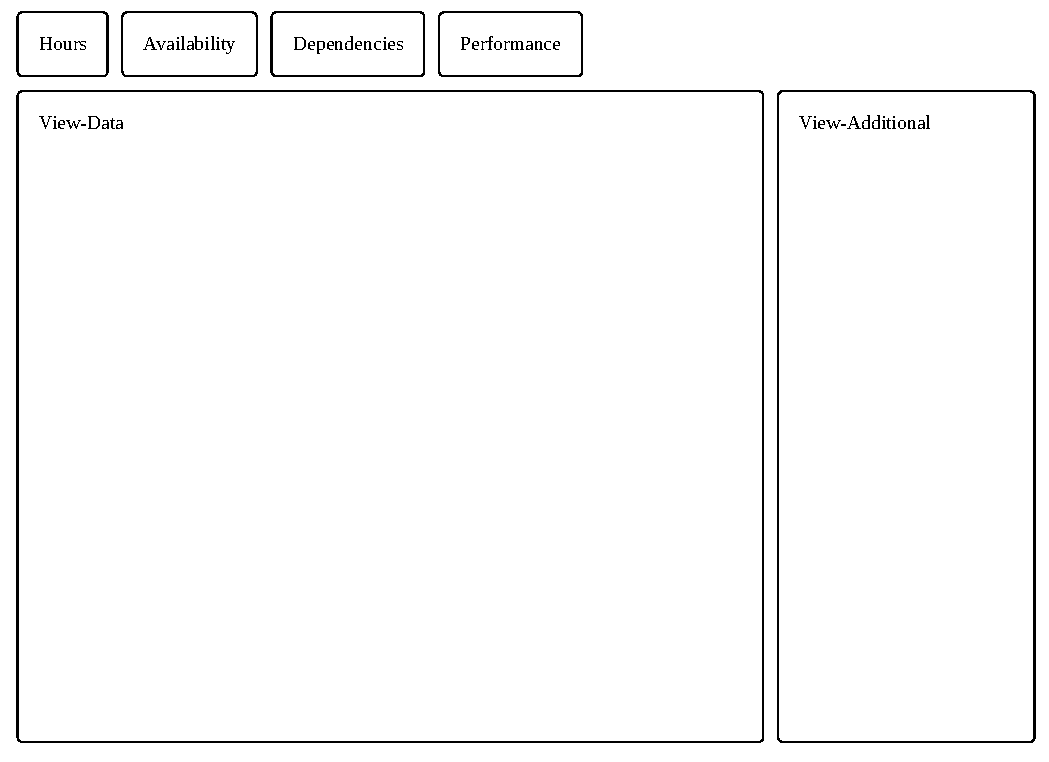
\includegraphics[valign=t,trim={.15cm .30cm .20cm .22cm},clip,width=.49\linewidth]{ui12.pdf}
		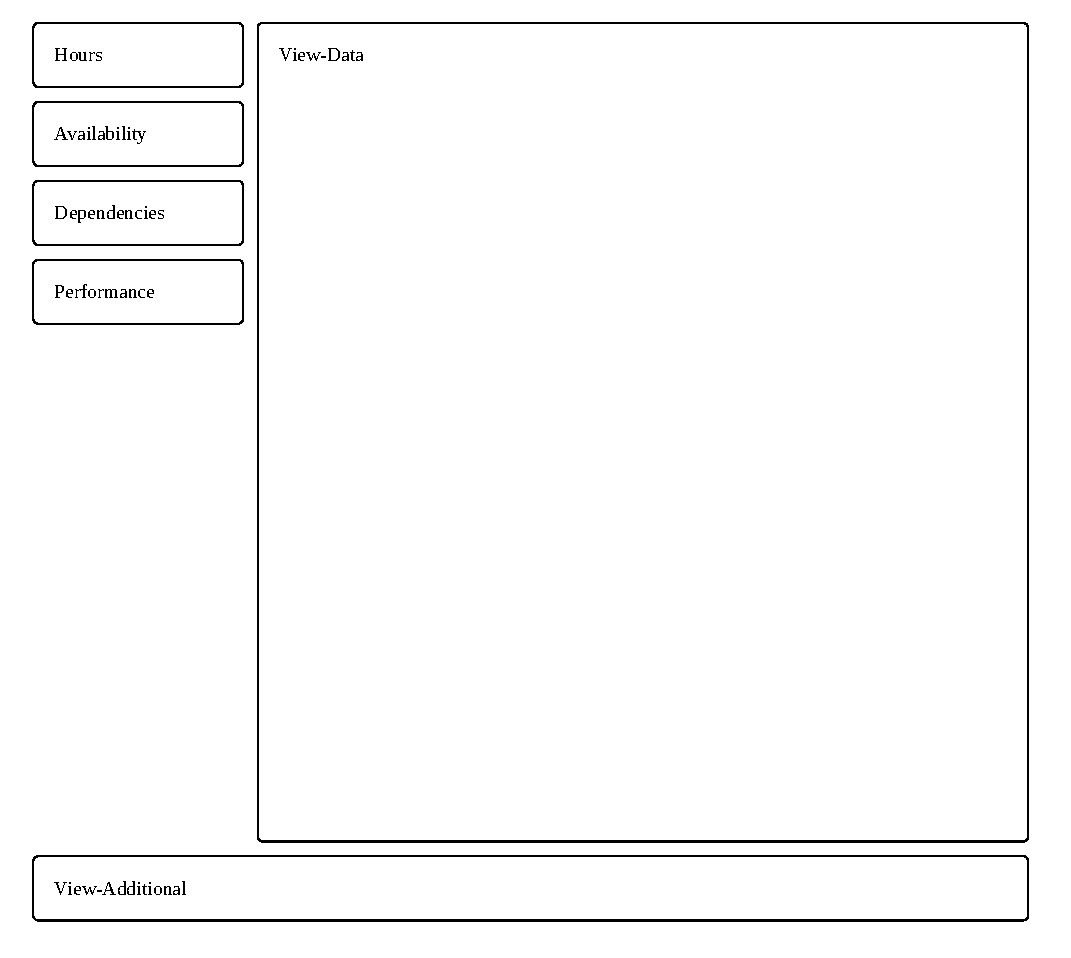
\includegraphics[valign=t,trim={.45cm .55cm .65cm .35cm},clip,width=.49\linewidth]{ui13.pdf}
		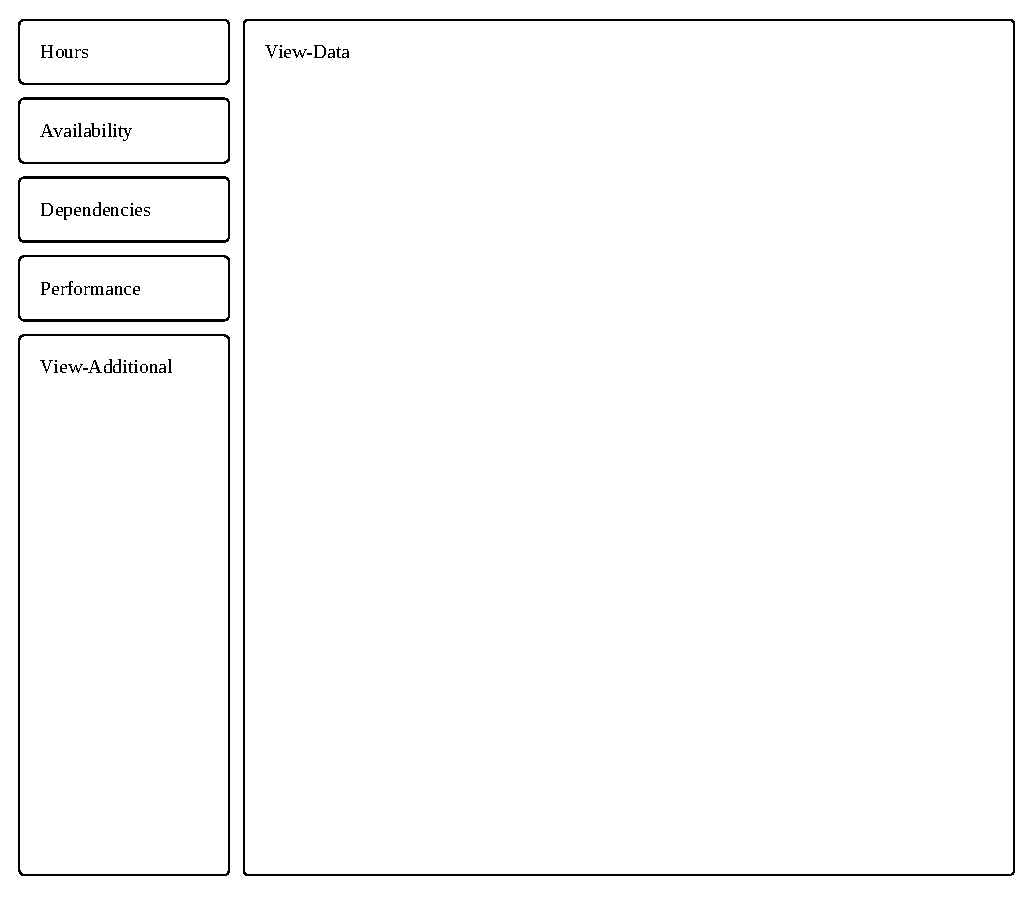
\includegraphics[valign=t,trim={.25cm .35cm .30cm .25cm},clip,width=.49\linewidth]{ui14.pdf}
		\caption{Design sketches 1.1, 1.2, 1.3 and 1.4}
		\label{label_mockupInterfaces}
	\end{figure}

	Since the task buttons represent our navigation, they were arranged either
	according to Krugs advice, either across the top or down the left side of a
	page. The placement of the \textit{View-Additional} was used as an additional
	permutation in order to create four design-sketches.

	Astute readers will undoubtedly notice that the presented designs do not
	feature colored buttons. Since the functionality of the design is explained
	to each interviewee at the start, it was decided that printing without colored
	buttons would be less distracting.

	\subsection{Interview-structure and sketch selection}

    The specific purpose of these interviews was to determine which of the
    presented ui-mockups was perceived to be the most usable.

    \begin{figure}[h!]
      \centering
      \includegraphics[trim={0 0 0 0},clip]{figures/lofi_method.pdf}
      \caption{Overall structure of prototype selection interviews.}
    \end{figure}

    The interviews were conducted in-person, with five team members, on
    the premises of Massive. The interview started with a description of
    what was happening; an evaluation of four different mock-up interfaces
    to determine which one was the most suitable for further testing.

    After confirming that there were no immediate questions, the
    interviewee was presented with the printed mock-ups in the same
    arrangement as shown in figure \ref{label_mockupInterfaces}. They were
    then asked to evaluate, out loud, the interfaces in any order they
    wished, and to ask if there was anything unclear about the assumed
    functionality.

    When the participant felt they were done and any questions they had
    about the interface were sorted out, they were asked to arrange the
    prototypes from best- to least-suited for the upcoming test purpose.
    Again, the participant was asked to voice their thought process out
    aloud as they did the sorting.

    After confirming that the interviewee was satisfied with their ordering, a
    set of ten flash-cards were introduced. These cards represent the combined
    key-words-attributes from ISO 9241-11\cite{citeISO9241} and ISO
    9241-12\cite{citeISO9241-12}, concerning usability and presentation of
    information respectively.

    Keyword definitions presented below:

        \begin{description}[style=nextline]
          \item[Effectiveness]{
            Usability is measured by the extend to which the
            intended goals of use of the overall system are achieved.
          }
          \item[Efficiency]{
            The resources that have to be expended to achieved the indented
            goals.
          }
          \item[Satisfaction]{
            The extent to which the user finds the overall system
            acceptable.
          }
          \item[Clarity]{
              The information content is conveyed quickly and accurately.
          }
          \item[Discriminability]{
              The displayed information can be distinguished
              accurately.
          }
          \item[Conciseness]{
              Users are not overloaded with extraneous information.
          }
          \item[Consistency]{
              A unique design, conformity with user's expectation.
          }
          \item[Detectability]{
              The user's attention is directed towards information
              required.
          }
          \item[Legibility]{
              Information is easy to read.
          }
          \item[Comprehensibility]{
              The maning is clearly understandable, unambiguous,
              interpretable, and recognizable.
          }
        \end{description}

    Where the top three terms are defined in ISO 9241-11 with the remainder
    coming from ISO 9241-12.

    In the next task, each participant was asked to order the keywords
    in order of how important they thought that specific quality was for a
    well-functioning, user interfacing software. There were no restrictions
    in regards to the number of times a participant could ask about the
    definition or clarification of each term.

    When the participant acknowledged that they were finished with their
    selection, they were asked to do one final task, to re-evaluate their
    previously selected ranking of the prototype interfaces, changing the order
    if they felt another one was more appropriate after being exposed to the
    ISO definitions.

    As for the final result of these interviews, all participants sans one,
    chose 1.4 as being the most usable in the initial ranking. And after the
    ISO definitions section everyones answered that 1.4 was the most suitable
    interface setup.

\section{Technology Stack}

  Since this is development-based project, this section will provide insight in
  why the different technology choices were made, and if any other
  choices were considered at the time.

  \subsection{Python}

  The backbone of the testing-platform is written in  Python\cite{citePython},
  a general purpose programming language that is steadily becoming
  more and more popular among developers according to the 2019 installment of
  the annual developer survey\cite{citeStackOverflow2019Survey},
  conducted by popular programming questions and answers site,
  StackOverflow\cite{citeStackOverflow}.

  In addition to the author having prior experience with Python, and the
  language being used heavily throughout Massive, the language
  is chosen due to its interesting relation to both data-analysis and
  web-development. When
  JetBrains\cite{citeJetBrains},
  creators of
  PyCharm\cite{citePyCharm},
  a Python coding environment, asked 24 000 Python
  developers:
  ``What do you use Python for?''\cite{citeJetSurvey}, allowing for multiple
  selections, 59\% answered data analysis and 51\% web development.

  Python is also the home of SciPy, ``a Python-based ecosystem of open-source
  software for mathematics, science and engineering''\cite{citeSciPyHomepage},
  that has become ``a de facto
  standard for leveraging scientific algorithms in
  Python''\cite{citeSciPyPaper}, making the language a good fit for gathering
  and processing data from studies in various ways.

  \subsection{Flask}

  Since one of the goals of this project is to facilitate usability-test in a
  geographically distributed team, presumably, over the internet, there
  needs to be web-component added to the mix. Here the final choice comes down
  down to Flask\cite{citeFlaskHomepage} or Django\cite{citeDjangoHomepage},
  two popular Python web-frameworks. Django facilitates an established
  structure and more features defined out-of-the-box, also known as ``batteries
  included'', while Flask encourages a more build-it-as-you-need-it approach.

  In the end Flask was chosen because it better supports the chosen iterative
  development process. Additionally, it is hard to know if the
  project-structure enforced by Django is a good fit or not until the
  development has been progressing for a while, which is not ideal when
  development resources are scarce.

  \subsection{SVG -- dynamic tasks, scaling and
  sharing}\label{label_svg_section}

  Scalable Vector Graphics (SVG) is, as described on the W3C-homepage, ``%
  \textit{%
    a markup language for describing two-dimensional graphics applications and
    images, [and is] \ldots supported by all modern browsers for desktops and
    mobiles.%
  }''\cite{citeW3CSVG}
  Where W3C stands for the World Wide Web Consortium, an international
  community that work together to develop web standards\cite{citeW3CHomepage}.

  While this choice might seem a bit odd for a reader that is somewhat versed
  in web-development, since it would undoubtedly be easier to visualize the
  user-interface using static images such as .png or .jpg, both common image
  standards used on the internet.

  However, there are specific advantages in using this markup language for this
  specific application. First, it is supported on a wide array of browsers and
  hardware, mitigating the loss of control of the underlying testing-hardware
  somewhat, more on this in section \ref{label_testingHardware}.

  Secondly, as stated in the name, this is a vector based graphics format.
  This means that the underlaying primitives are made up by  points and vectors
  instead of pixels storing color values. This approach enables the interface
  scale very well, both to larger and smaller formats, without any loss of
  quality. The usability of such a scaled interface of course assumes that the
  underlying interface design is done in such a way that it will still be
  usable at the new size, but there is no need to take concerns about loss of
  quality into account.

  The third point is closely related to the second point. Since all the
  graphical information of the page will be displayed using this vector format,
  making a high-fidelity sharable snapshot of the current state of the page is
  as easy as printing the page to a pdf through the standard print-dialog in
  the browser viewing the page. At the time of writing, this works best
  in Googels popular web-browser, Chrome, and is the method used to produce all
  figures visualizing the platform in the following sections, feel free to zoom
  in on any of them if you are reading this in a digital format.

  Lastly, since the format is text-based, it is possible to use any programming
  language that can handle text, Python in this case, to dynamically generate
  interfaces wholesale or to apply modifications, such as randomization or
  parameters-adjustment on already existing base-interfaces on the fly.

\section{Potential primary users}

	Around this point in the process it became clear that the result from this
	project would be a little rough around the edges, as opposed to a one-press
	solution for remote web-based usability testing. The final goal would be to
	push it to such a degree of usability that a designer that knows nothing
	about web-development or python could setup some remote user-tests and gather
	usable data from users through the internet.

	As it stands, getting the platform up and running needs the input of an
	individual or team that has some degree of familiarity with python, flask and
	web-development. Though this is a higher barrier to entry than the final goal
	above, it would still be suitable for a testing-engineer with some
	web-background, possibly in academia or game-development.

\section{Sketch implementation}

%\todo{Här saknas beskrivning av din prototyp/ditt system. Du beskriver
%testupplägg och tasks men inte själva utformningen av prototypen. Lägg till det
%(eller flytta om ordningen i texten då det kanske kommer lite längre fram i
%3.4.3->).}
%
%\todo{Fundera också på begreppet hifi prototype, kan mycket väl passa
%bra men fundera igenom det.}
%
%\todo{Det som rör till det lite extra är att ni
%prototypar inte bara en plattform för webbaserad testning utan samtidigt ett
%system för att kolla workload, etc. Du behöver skriva fram tydligare hur du
%tänker kring dessa två. Jag tror det viktigaste är strukturen för webbaserad
%testning, medan innehållet (workload etc) bara är skapat för att ha något
%relevant att testa på och inte är lika centralt.}

%  \subsection{Landing page}
%
%  After the participant has submitted the pre-survey, it  disappears and is
%  replaced by a few basic statistics about the current test session.
%  The functionality of the left-side buttons is restored and makes it
%  possible to choose any of the following four test types:
%  \textit{Employee Hours},
%  \textit{Team Workload},
%  \textit{Task Dependencies} and
%  \textit{Team Performance}.

	Here is a capture of the implementation of the chosen design sketch, running
	in a browser, the current state is past the consent-form and after the
	pre-survey has been submitted.

	\begin{figure}[h!]
		\centering
		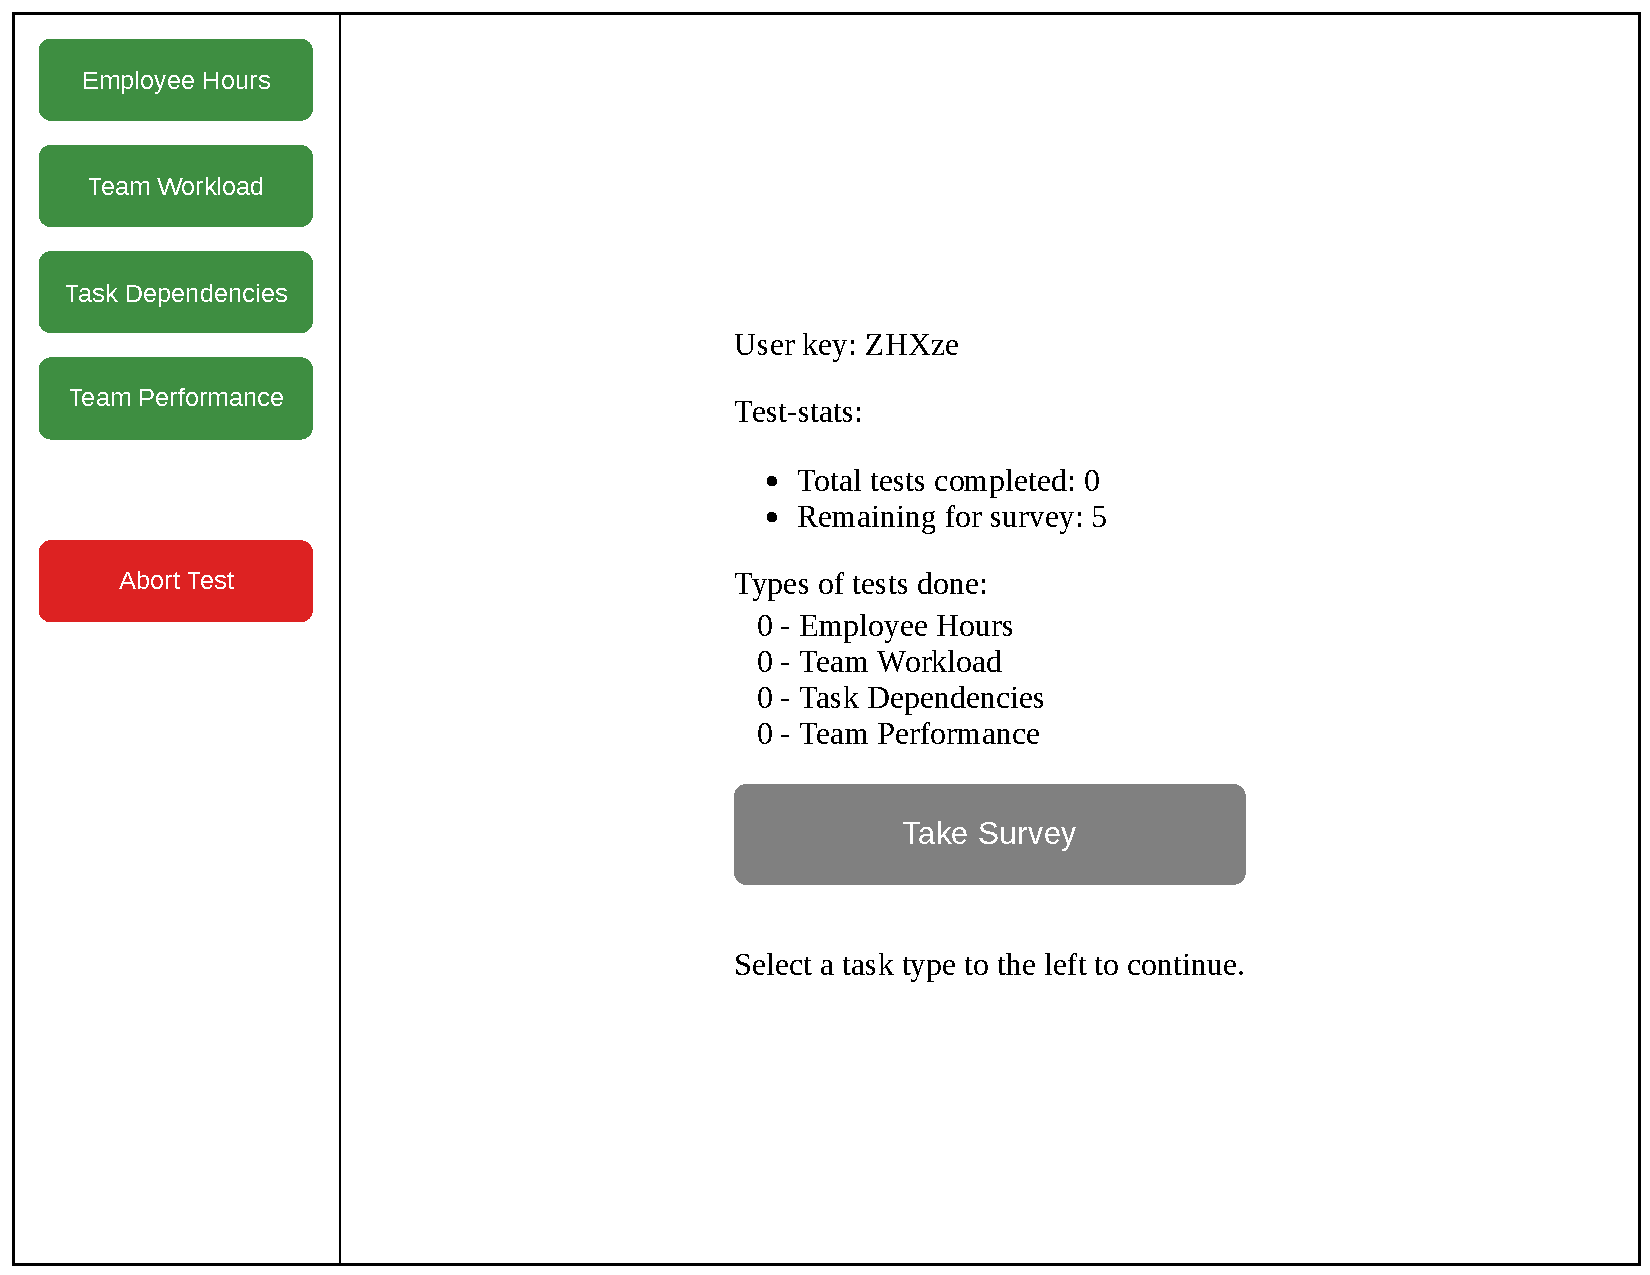
\includegraphics[width=.7\textwidth]{figures/captures/webapp_main_statistics.pdf}
		\caption{Capture of implementation of the chosen sketch.}
		\label{label_mainStatistics}
	\end{figure}

	It is worth noting that the \textit{View-additional} component has been
	removed due to none of the currently running tasks needing more advanced
	inputs. This space is instead used to host the Abort Test button, which will
	be explained in the following pages.

	When accessing the test for the first time, the participant is greeted by a
	information and consent screen, detailing the goals of the test and how the
	information generated by their activity will be used. The full information
	and consent page can be found in figure \ref{label_infoConsent}.

  Participants that accept and submit the consent form are then redirected
  to the main landing page. This page acts as a hub for the duration of
  the test session, providing access to all other parts of testing
  application. On the first visit the main view of the landing page is
  occupied by the initial survey, shown below, with a larger version available
  in figure 8.6 in the appendices.

  \begin{figure}[h!]
    \centering
    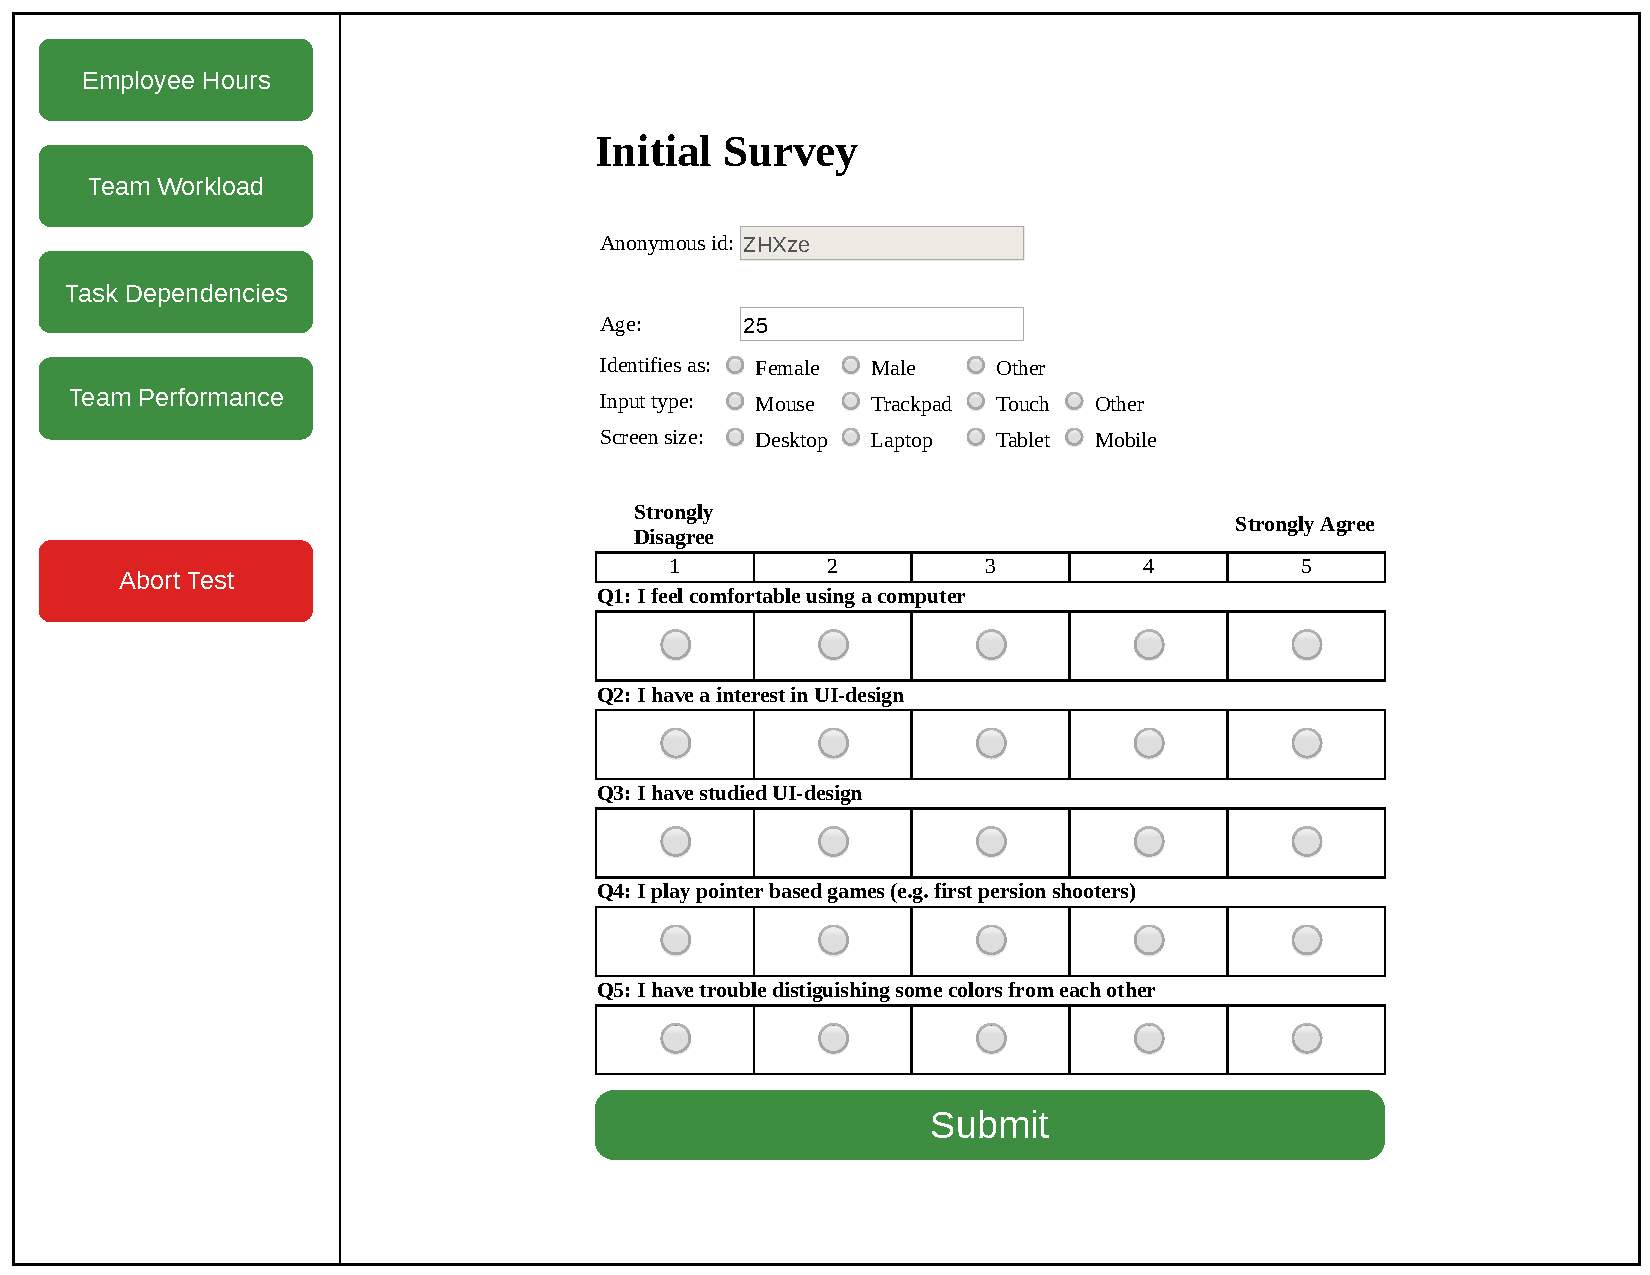
\includegraphics[width=.65\textwidth]{figures/captures/webapp_pre_survey.pdf}
    \caption{Capture of initial survey page.}
    \label{label_preSurvey}
  \end{figure}

  While it is possible for the participant to interact with the buttons on
  the left side before the initial survey is submitted, clicking any of the
  buttons except 'Abort Test' will only display the same survey-page.

  \begin{figure}[h!]
    \centering
    \fbox{
      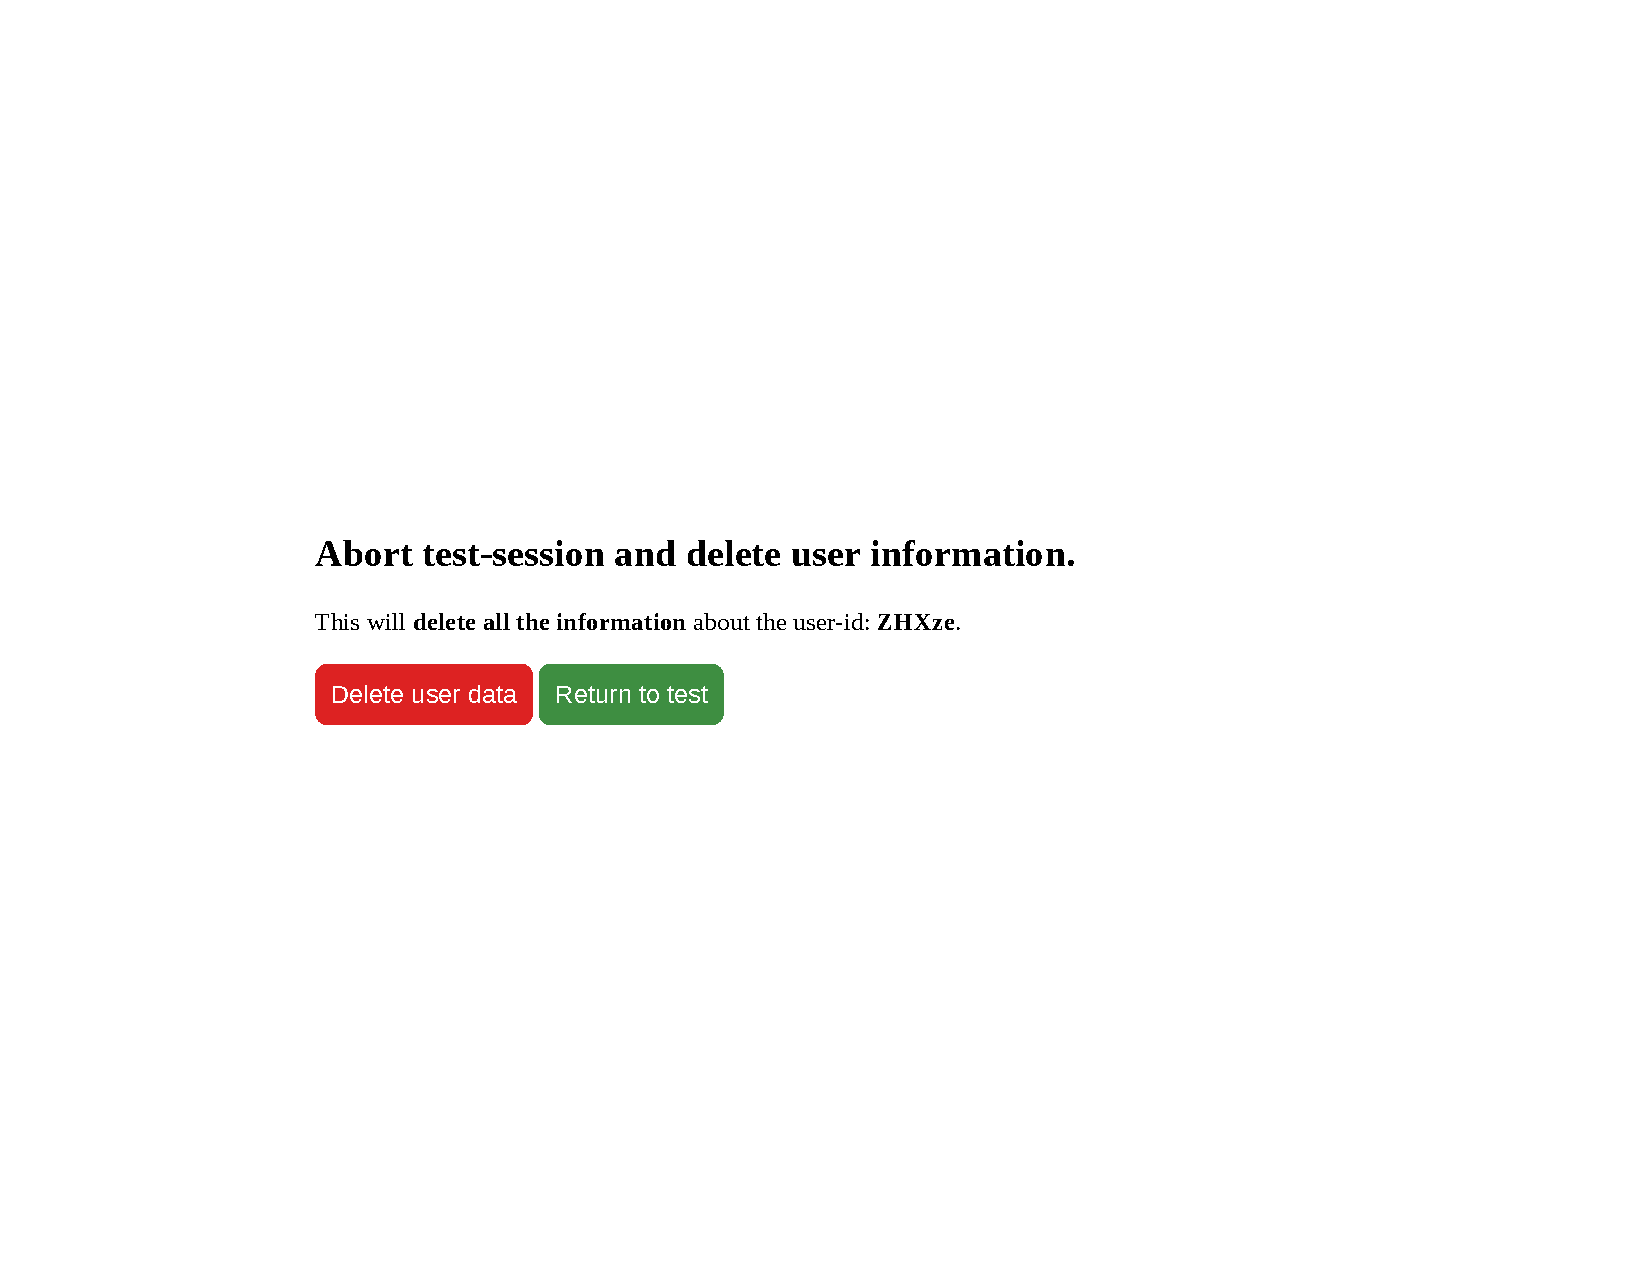
\includegraphics[trim={4cm 8cm 9cm 8cm},clip,width=.5\textwidth]{figures/captures/webapp_abort.pdf}
    }
    \caption{Capture of confirmation page for aborting the test.}
    \label{label_abort}
  \end{figure}

  The dedicated 'Abort Test' button is available in all the different
  views of the application, in case the participant no longer wants to
  participate for any reason. Clicking this button displays a page
  explaining that continuing will scrub any activity related to their
  current anonymous id from the database and abort the current test.
  %Additionally and return it to the pool
  %of available identification strings.

  %While the choices for the input method, except the last one, corresponds
  %directly to a concrete input method used in human-computer interactions, the
  %screen-sizes are somewhat ambiguous. This was an active choice in order to
  %not alienate participants by forcing them to specify an actual measurement
  %for the screen size. The assumed values for the screen-sizes ranges for the
  %given choices are:
  %\textit{Desktop} $>$17",
  %\textit{Laptop}  12"-17",
  %\textit{Tablet}  7"-12" and
  %\textit{Mobile}  $<$7".

%  \subsection{Post survey}

%  \todo{Även här blandar du lite mellan utvärdering av det webbaserade
%  systemet för testning (om uppgifterna var tydliga tex) och själva
%  utformningen av innehållet (om färgerna spelade roll). Du får i text försöka
%  förtydliga denna blandning av fokus genom rapporten. }

	\newpage
		As the participant completes five or more tests the 'Take Survey' button,
		seen in figure \ref{label_mainStatistics}, goes from gray to green,
		signaling that it has become active. Clicking this button redirects the
		participant to the post-survey page, other than the survey itself, there is
		also the option to return to the tests if the button was pressed by
		accident or if the participant has changed their mind.

		The post-survey consist of eight questions regarding both the test-platform
		and the test-tasks. Event though the main development focus is on the
		testing-platform it is still interesting to get some initial insight into
		how the participants felt about the test tasks in order to make them as
		user-friendly as possible in later iterations.

    \begin{figure}[h!]
      \centering
      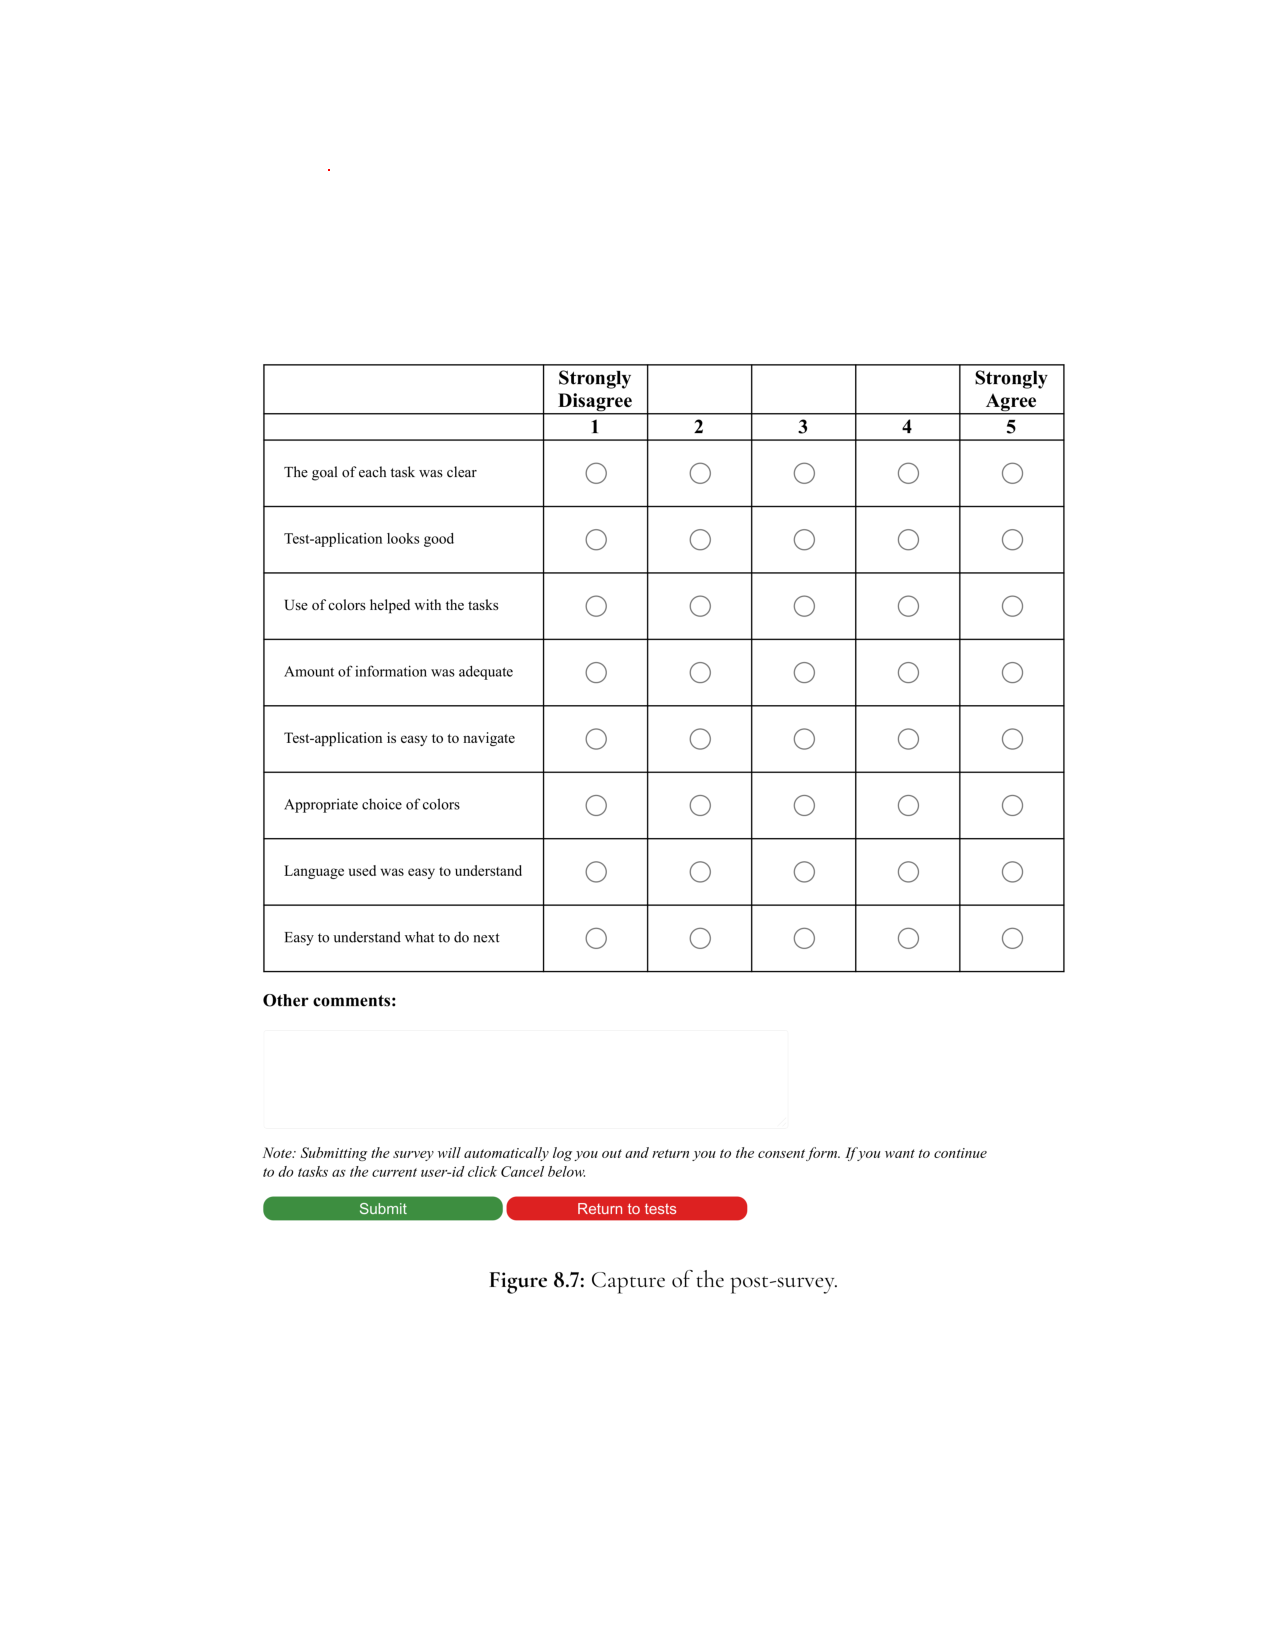
\includegraphics[trim={2.0cm 4cm 2.0cm 5cm},clip,width=.7\textwidth]{figures/captures/webapp_post_survey.pdf}
      \caption{Capture of the post-survey.}
    \end{figure}

    %Options that are of interest include, among others, if the goal of each
    %task was clear, if the application was pleasing to look at, if the use of
    %colors help when navigating application, etcetera. For
		A larger version of the capture is available as figure 8.7 in the appendices.

\subsection{Flow of a test-sessions and test-tasks}

	In order to properly begin the implementation of the back-end logic for the
	platform, the general test-flow for each participant has to be defined. This
	is done using the high-level description of a test
	method\cite[p.78]{citeHandbookUsability} as inspiration with some
	modifications due to the remote nature of the tests.

  \begin{figure}[h!]
    \centering
    \includegraphics{figures/test_flow.pdf}
    \caption{Illustrated flow for overall test-session.}
  \end{figure}

  The first major difference is the overall lack of time-limits. Since these
  tests are performed online, at a device of the participants choice at a,
  presumably, fitting time for them there is really no resource-restrictions in
  play as for how long a individual test-session could be. There is however a
  restriction centered around the minimum allowed tests performed, since in
  order to measure performance and the effects of repeated tests there needs to
  be a minimum number of tests performed by each participant.

  Other than this, the overall test-flow follows the basic outline, beginning
  with a nondisclosure and privacy statement (Information and consent),
  followed by a combined background and experience questionnaire (Pre-survey).
  Then in order to complete the test-flow, a participants completes at least
  five tasks of their choosing, more if they want, ending with a post-test
  debriefing (Post-survey). Again, with the main difference being the absence
  of an active moderator, due to the online nature of the tests.

  \begin{figure}[h!]
    \centering
    \includegraphics{figures/test_flow_task_runs.pdf}
    \caption{Illustrated flow for individual task-runs.}
  \end{figure}

  As for the flow of each individual tasks, it is split into three distinct phases;
  \textit{Task selection},
  \textit{Task-Info} and
  \textit{Task-Execution}.
  Each of the sections final design, purpose and implementation is
  described in greater detail in later sections below.

  What is worth noting here is that, as with many of the other steps, the
  participant is free to spend any amount of time on the first and second
  section, moving between them freely. It is when moving to the last stage,
  execution that the interface becomes more restrictive, locking the
  participant into the selected task, and measuring the time to the first
  submitted answer regardless if it is correct or not.

\section{The test-tasks}

	This section takes a closer look at the design of the test-tasks being tested
	on the implemented platform. The goal of each task is to find an specific
	element and click it as fast as possible. The reasoning behind using time to
	completion as the main metric for these tasks was that it is a value that is
	relatively easy to measure precisely enough over the internet. Additionally,
	when used in this context it provides an clear success-criteria, faster is
	better.

  \subsection{Employee hours}

		The premise of this task is that there exists multiple assignable tasks, each
		with a pre-determined cost. These tasks can then be assigned to employees
		that have a finite pool of work-hours, making it possible to over-assign a
		employee.

    \begin{figure}[h!]
      \centering
      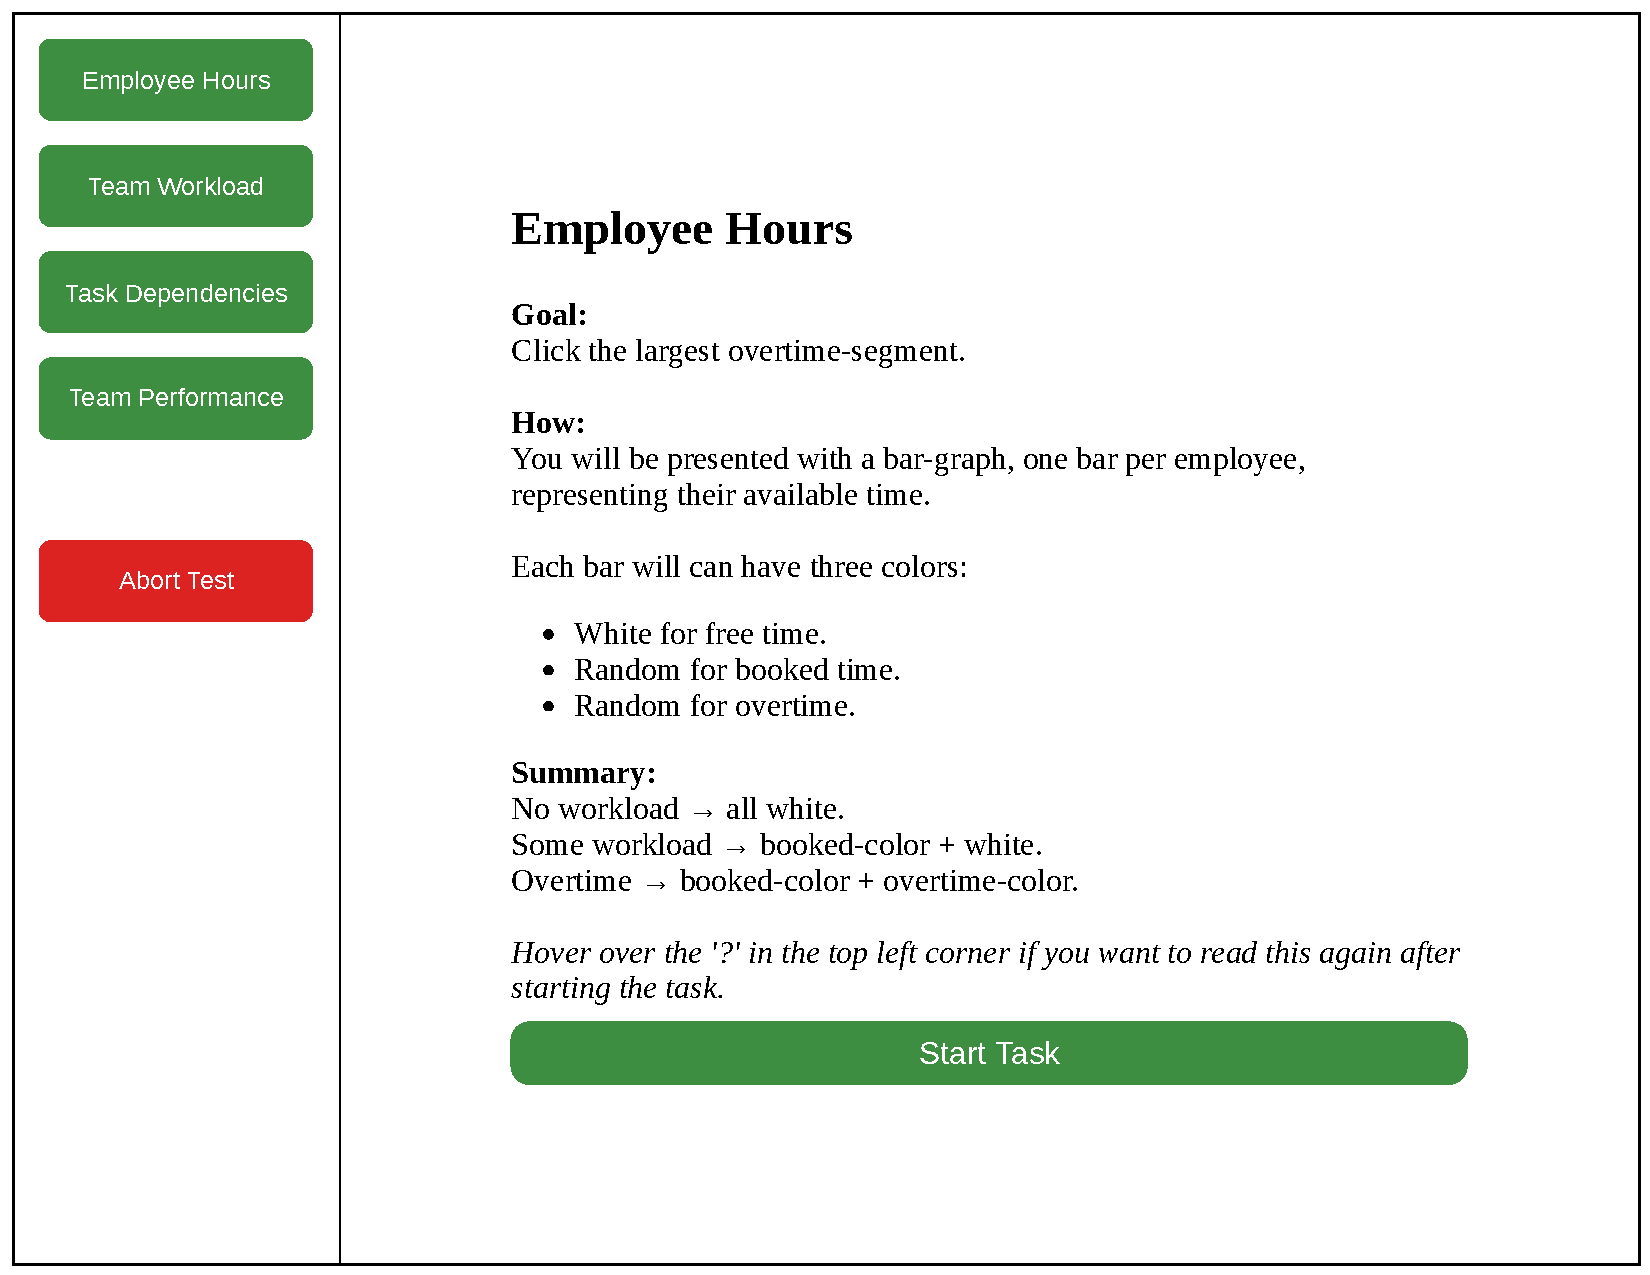
\includegraphics[width=.49\textwidth]{figures/captures/webapp_employee_hours_info.pdf}
      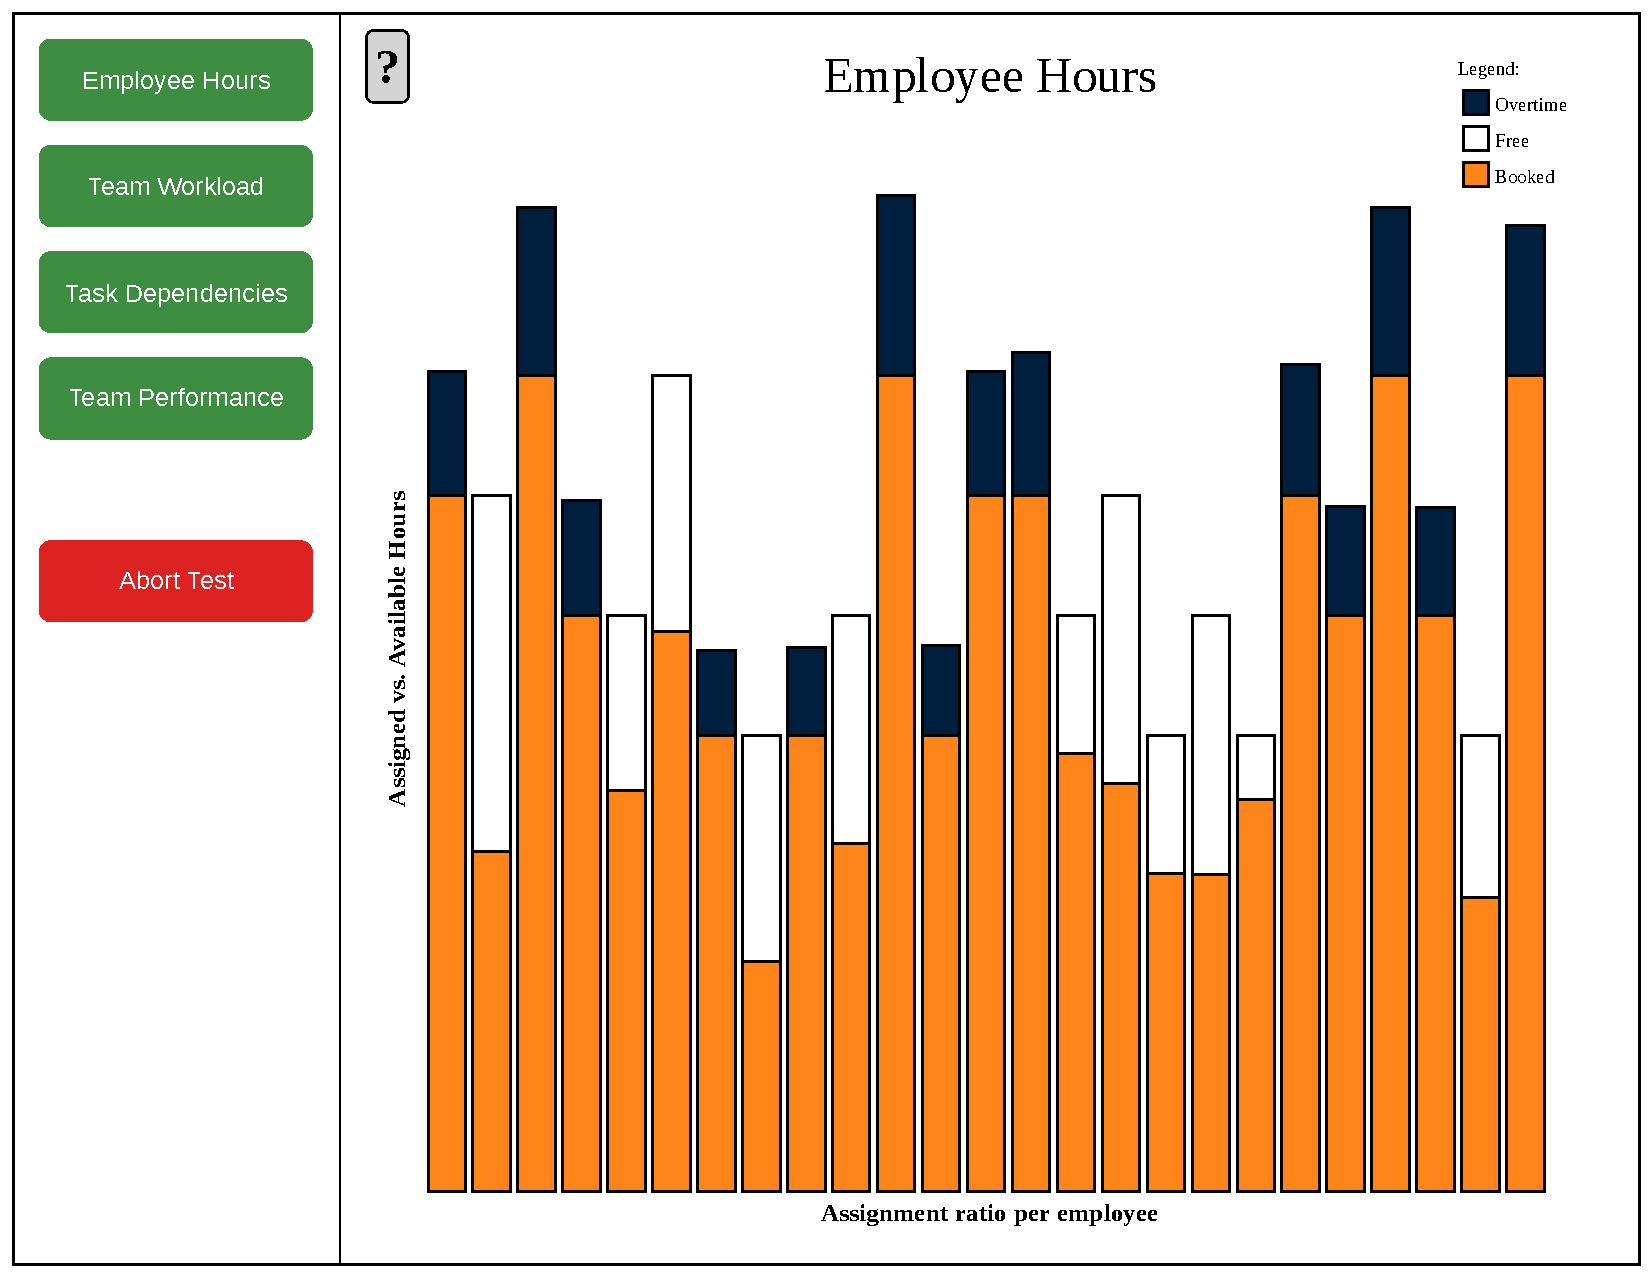
\includegraphics[width=.49\textwidth]{figures/captures/webapp_employee_hours_task.pdf}
      \caption{Capture of Employee Hours information and task page.}
    \end{figure}

		The goal of this tasks is to find out, as fast as possible, which of the
		employees, represented by the bars, is the most over-scheduled one. This is
		done by identifying and selecting the largest black segment. White segments
		signal that there is work-capacity left, and these bars can be safely
		ignored.

  \subsection{Team workload}

		This test task simulates a work-calendar where the saturation of the color
		in each cell represents the amount of work that needs to get done during
		that particular day.

    \begin{figure}[h!]
      \centering
      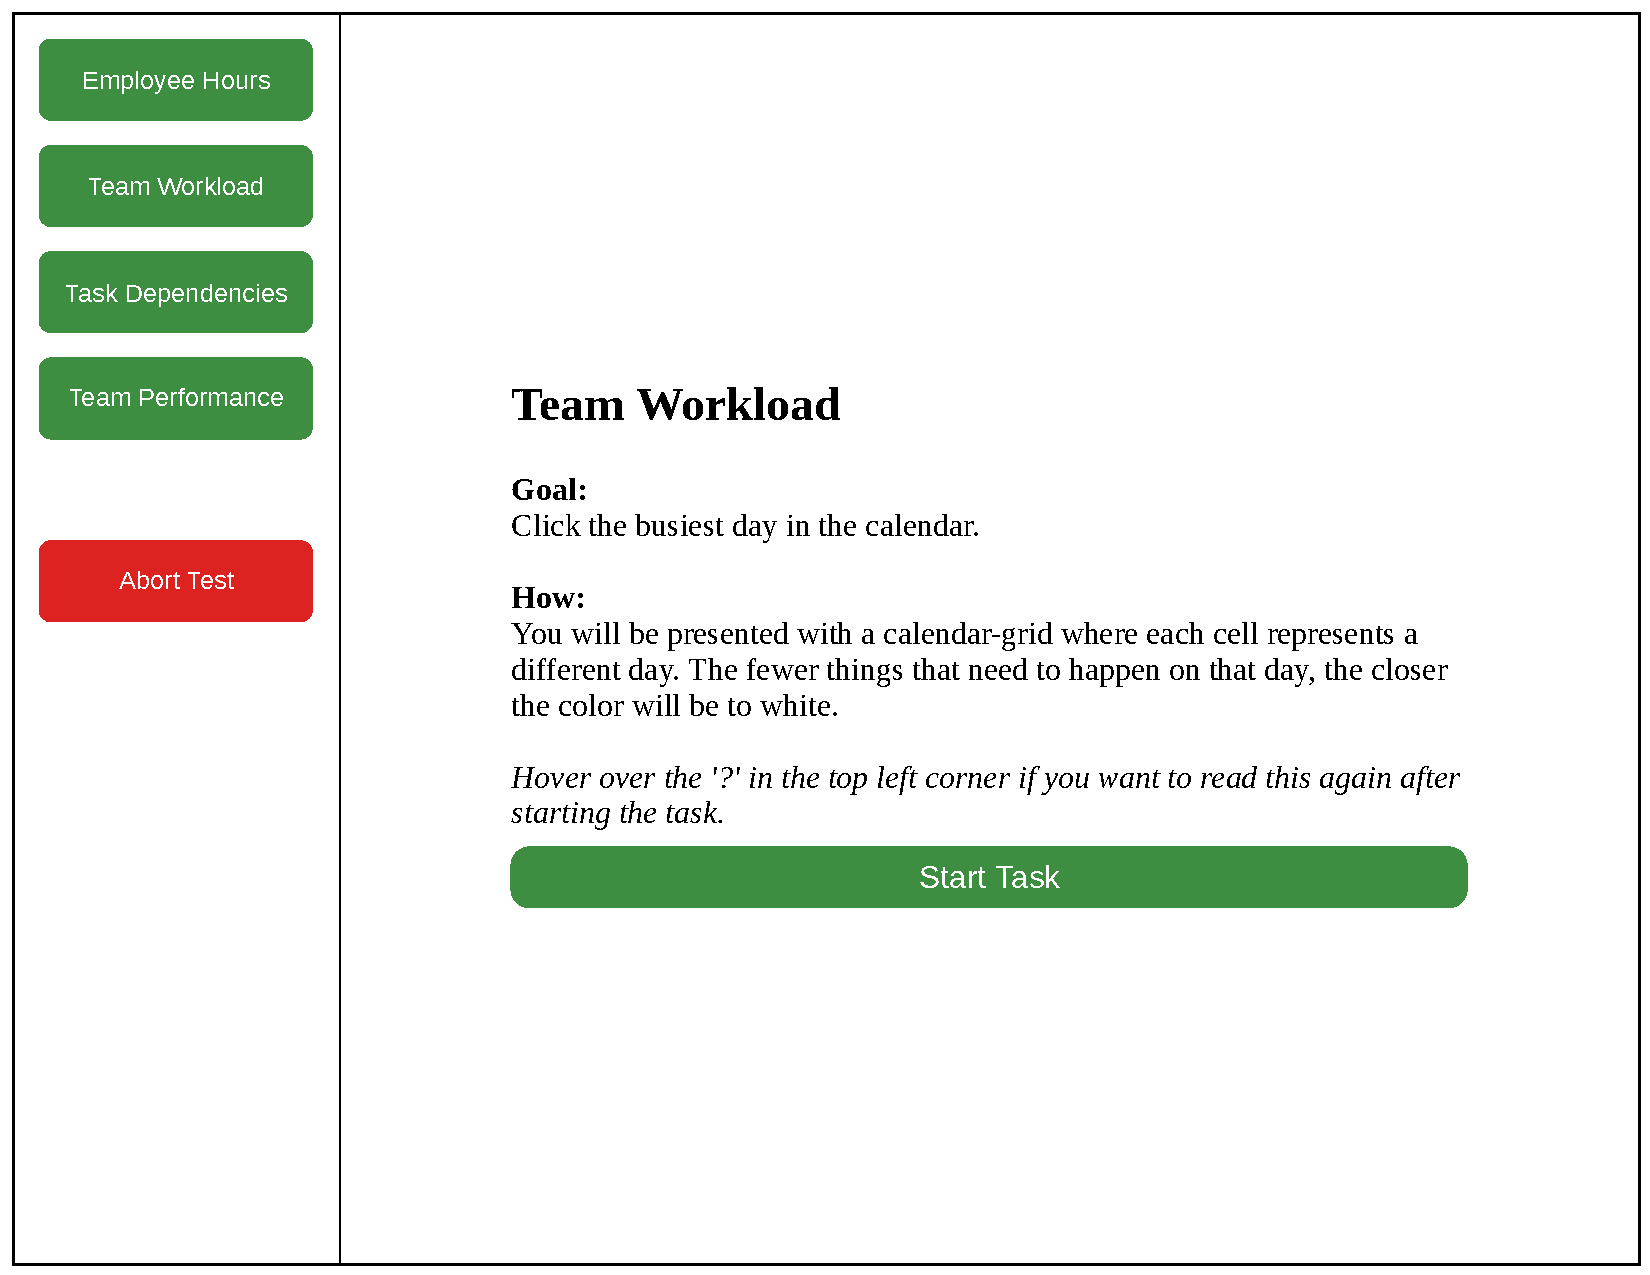
\includegraphics[width=.49\textwidth]{figures/captures/webapp_team_workload_info.pdf}
      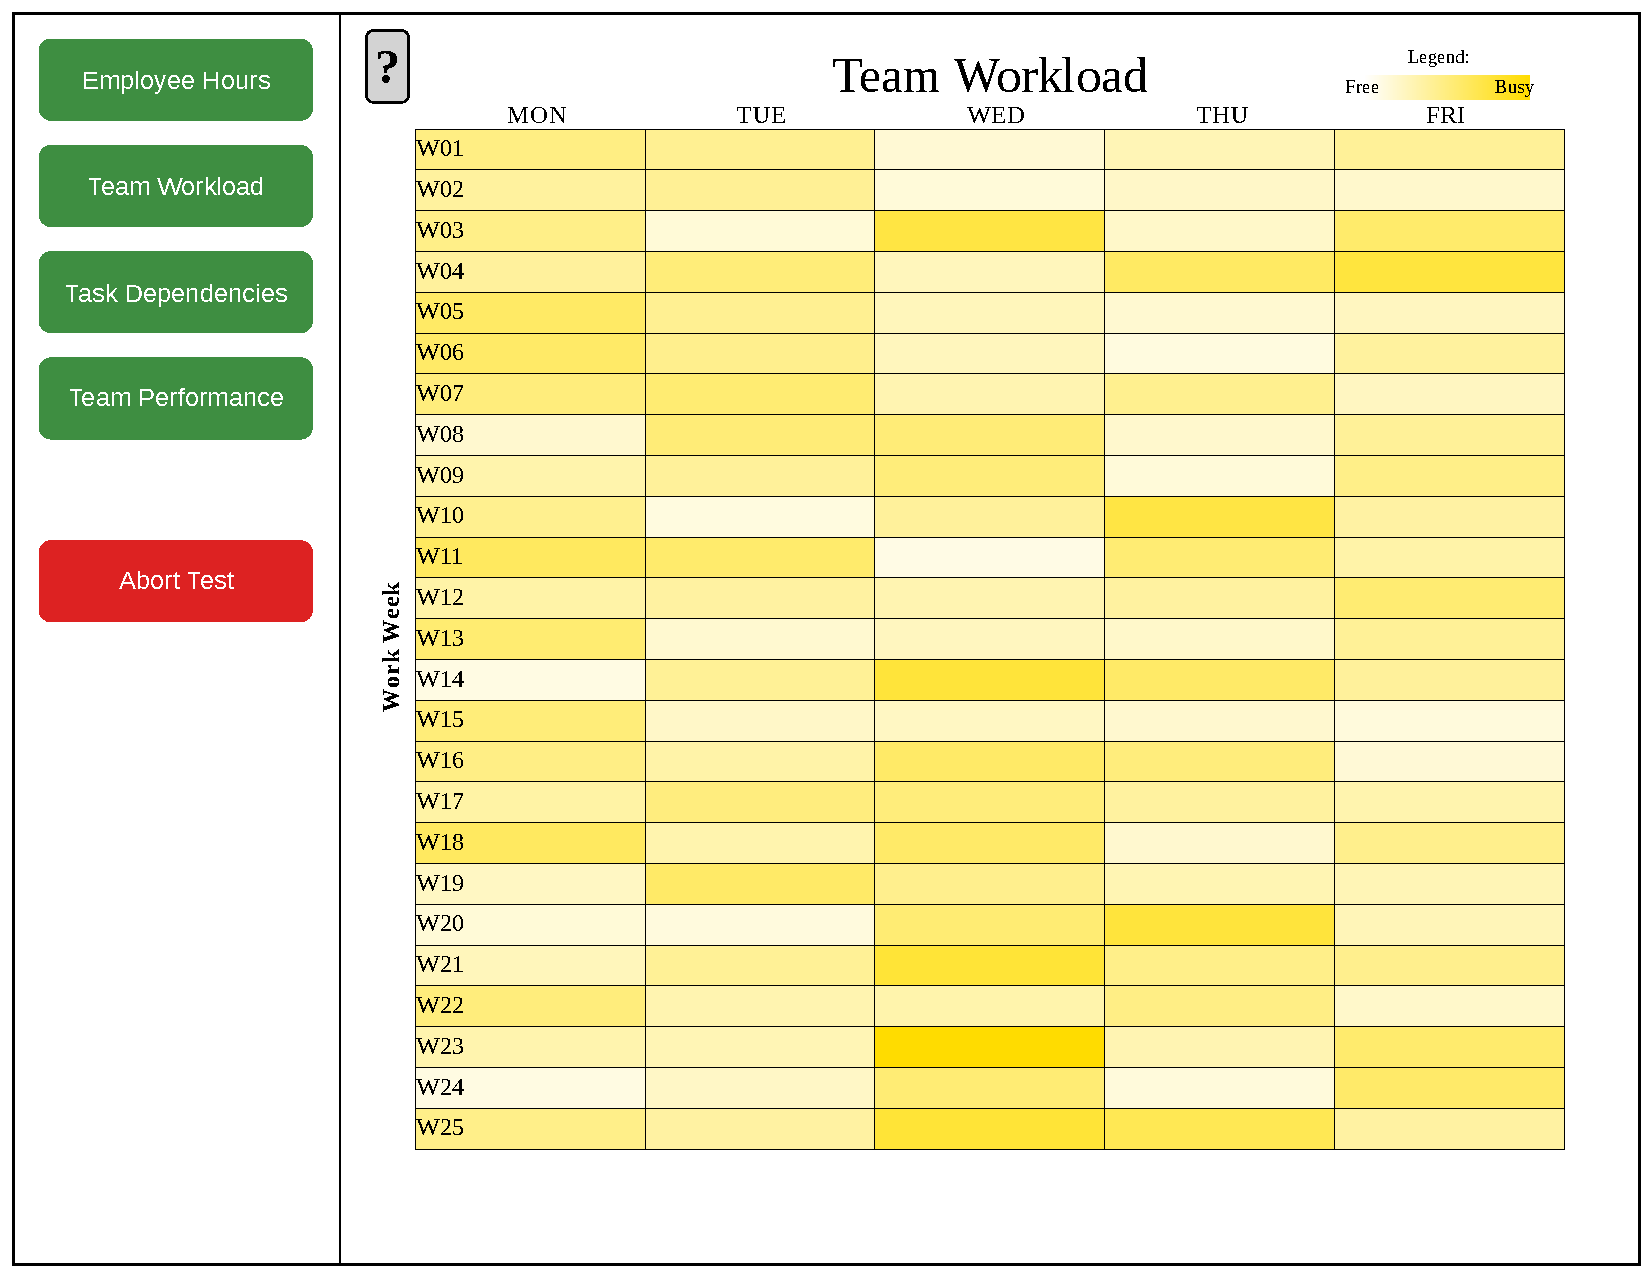
\includegraphics[width=.49\textwidth]{figures/captures/webapp_team_workload_task.pdf}
      \caption{Capture of Team Workload information and task page.}
    \end{figure}

		Here the goal is to identify which of the days that is the busiest, which
		in this case is equal to the cell with the darkest color, and click on
		that, as fast as possible.

  \newpage
  \subsection{Task dependencies}

		Sometimes there are tasks that need to be completed before the next set of
		tasks can be started, this is a simulation of that type of dynamic.

    \begin{figure}[h!]
      \centering
      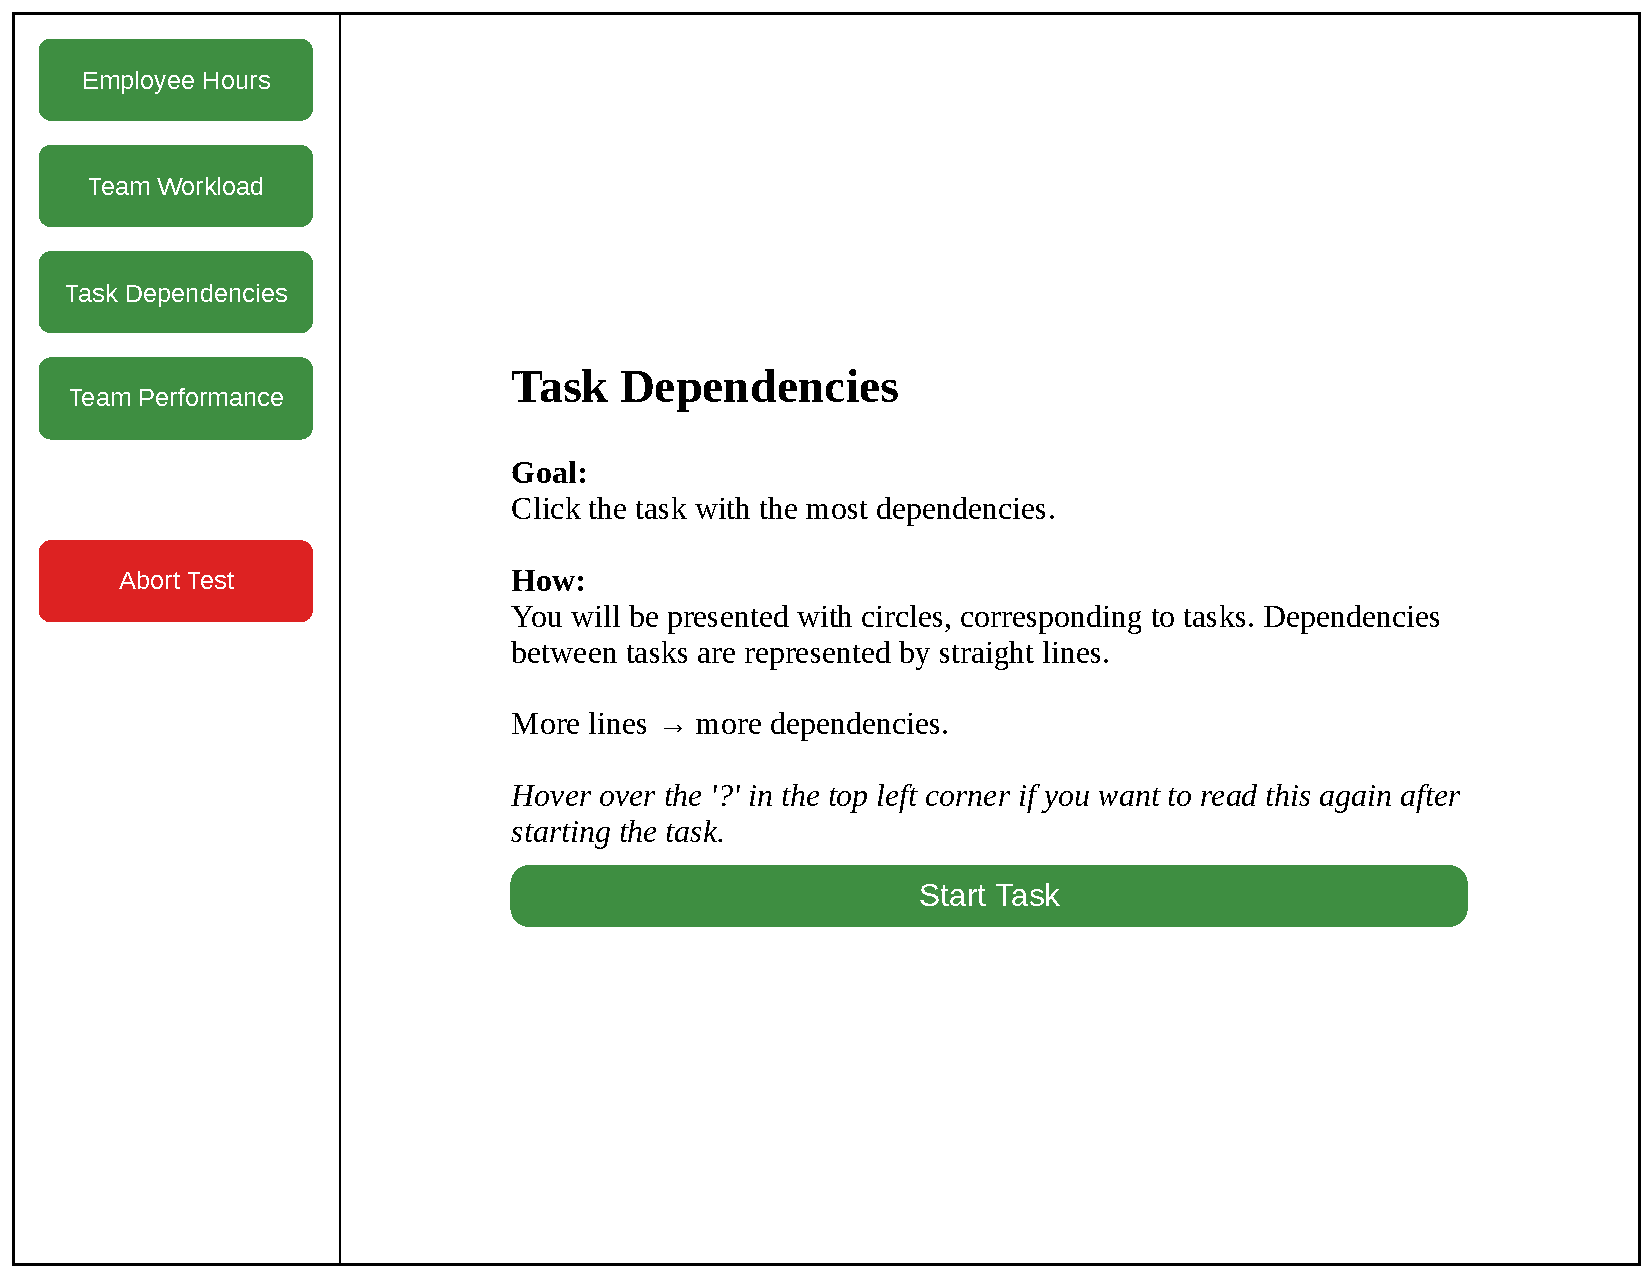
\includegraphics[width=.49\textwidth]{figures/captures/webapp_dependencies_info.pdf}
      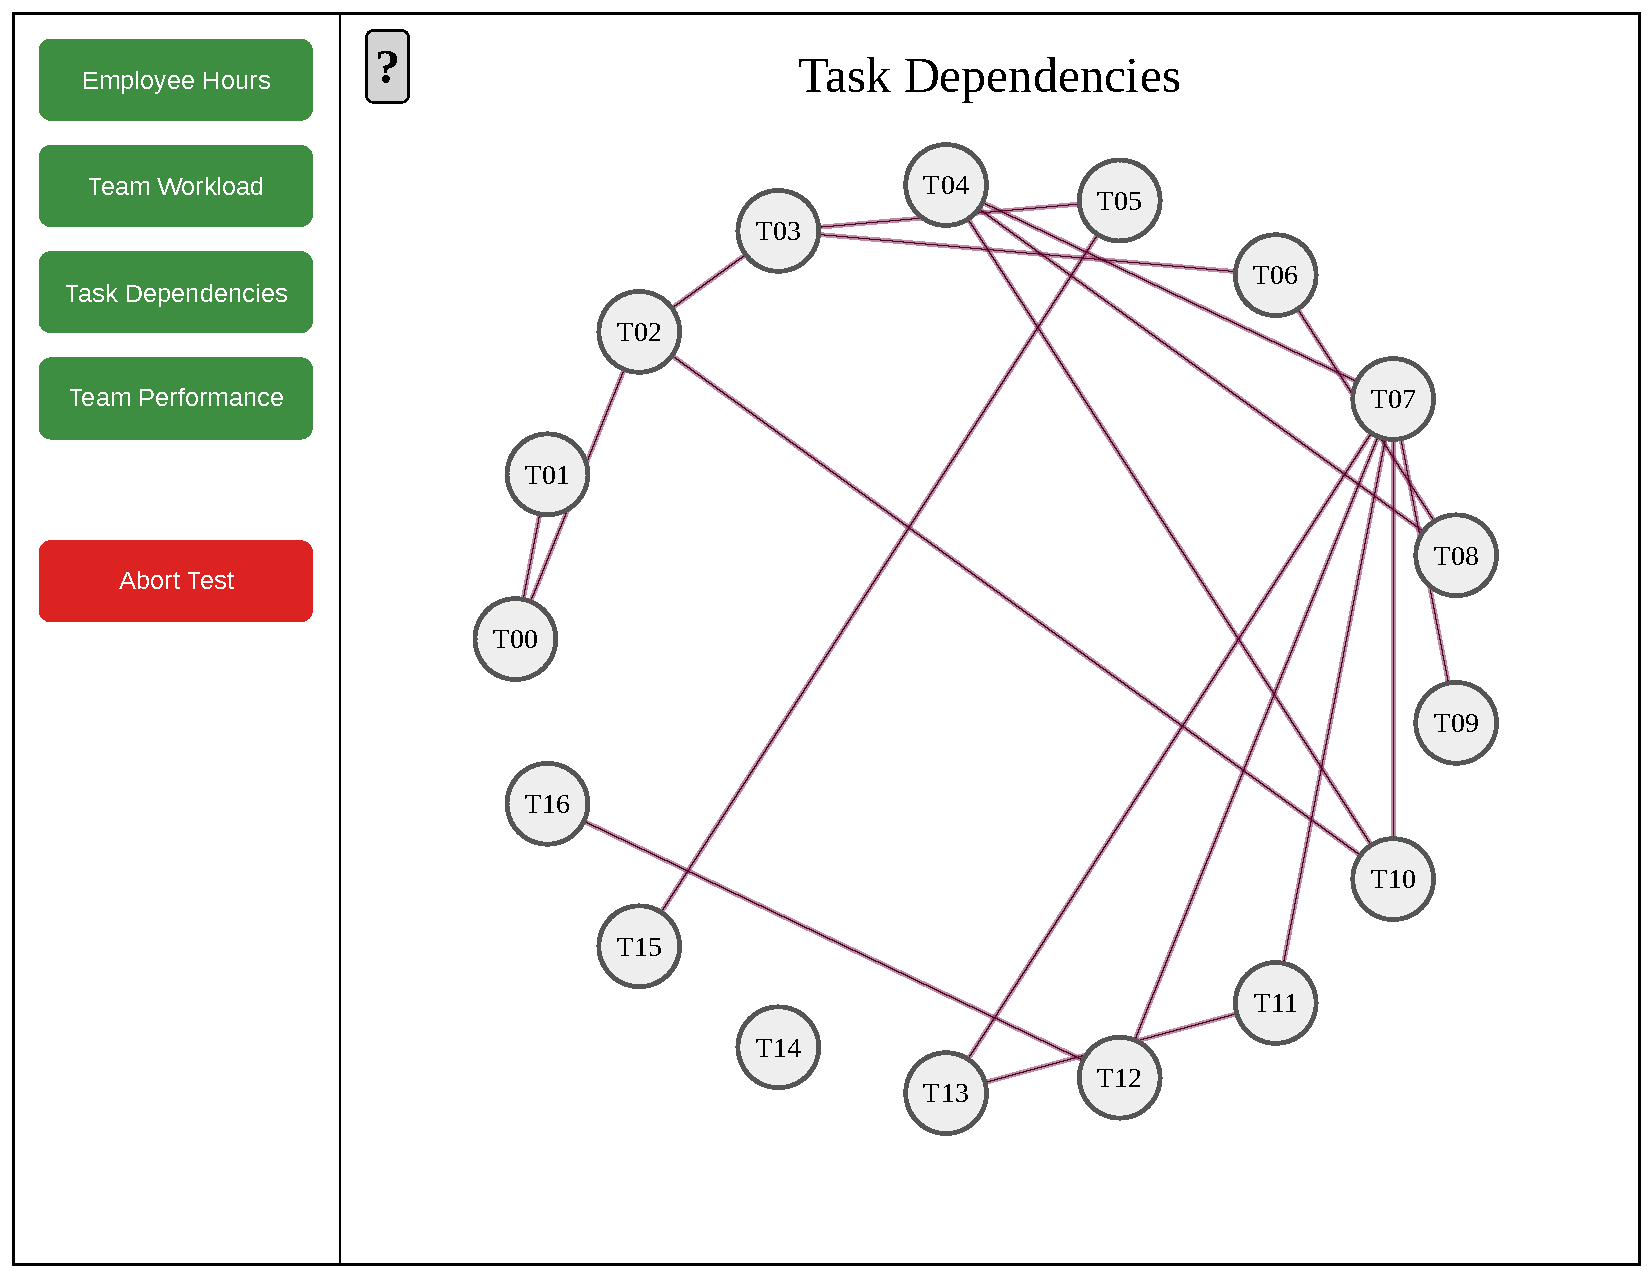
\includegraphics[width=.49\textwidth]{figures/captures/webapp_dependencies_task.pdf}
      \caption{Capture of Task Dependencies info- and task-page.}
    \end{figure}

		Each of the seventeen circles represents a tasks, and the lines between
		them represents an dependency with unspecified direction. The goal of the
		task is to find the most connected circle and click it, again, as fast as
		possible.

    \subsection{Team performance}

		Everyone has things they are better at doing than other things. In this
		task there are seven teams, represented by the vertical bars. Within these
		bars are further segmentations, representing different types of tasks.

    \begin{figure}[h!]
      \centering
      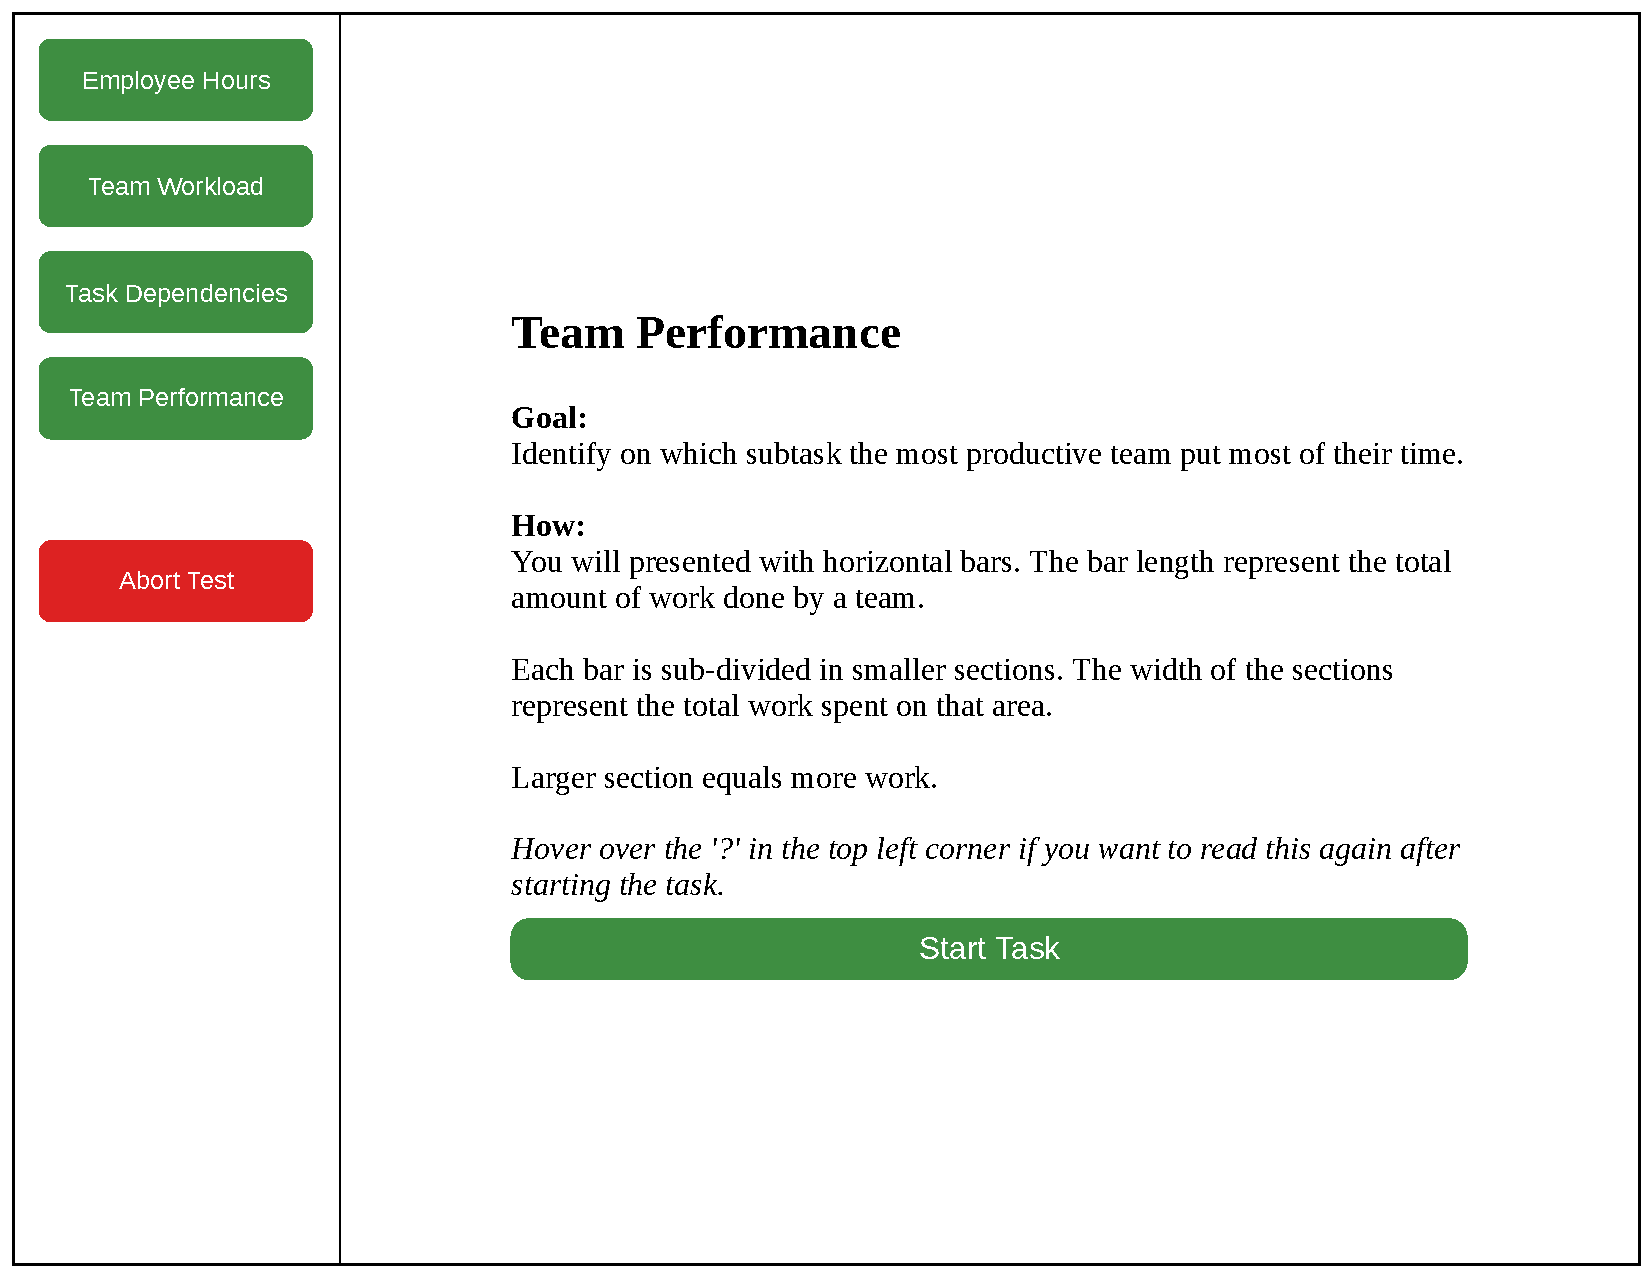
\includegraphics[width=.49\textwidth]{figures/captures/webapp_team_performance_info.pdf}
      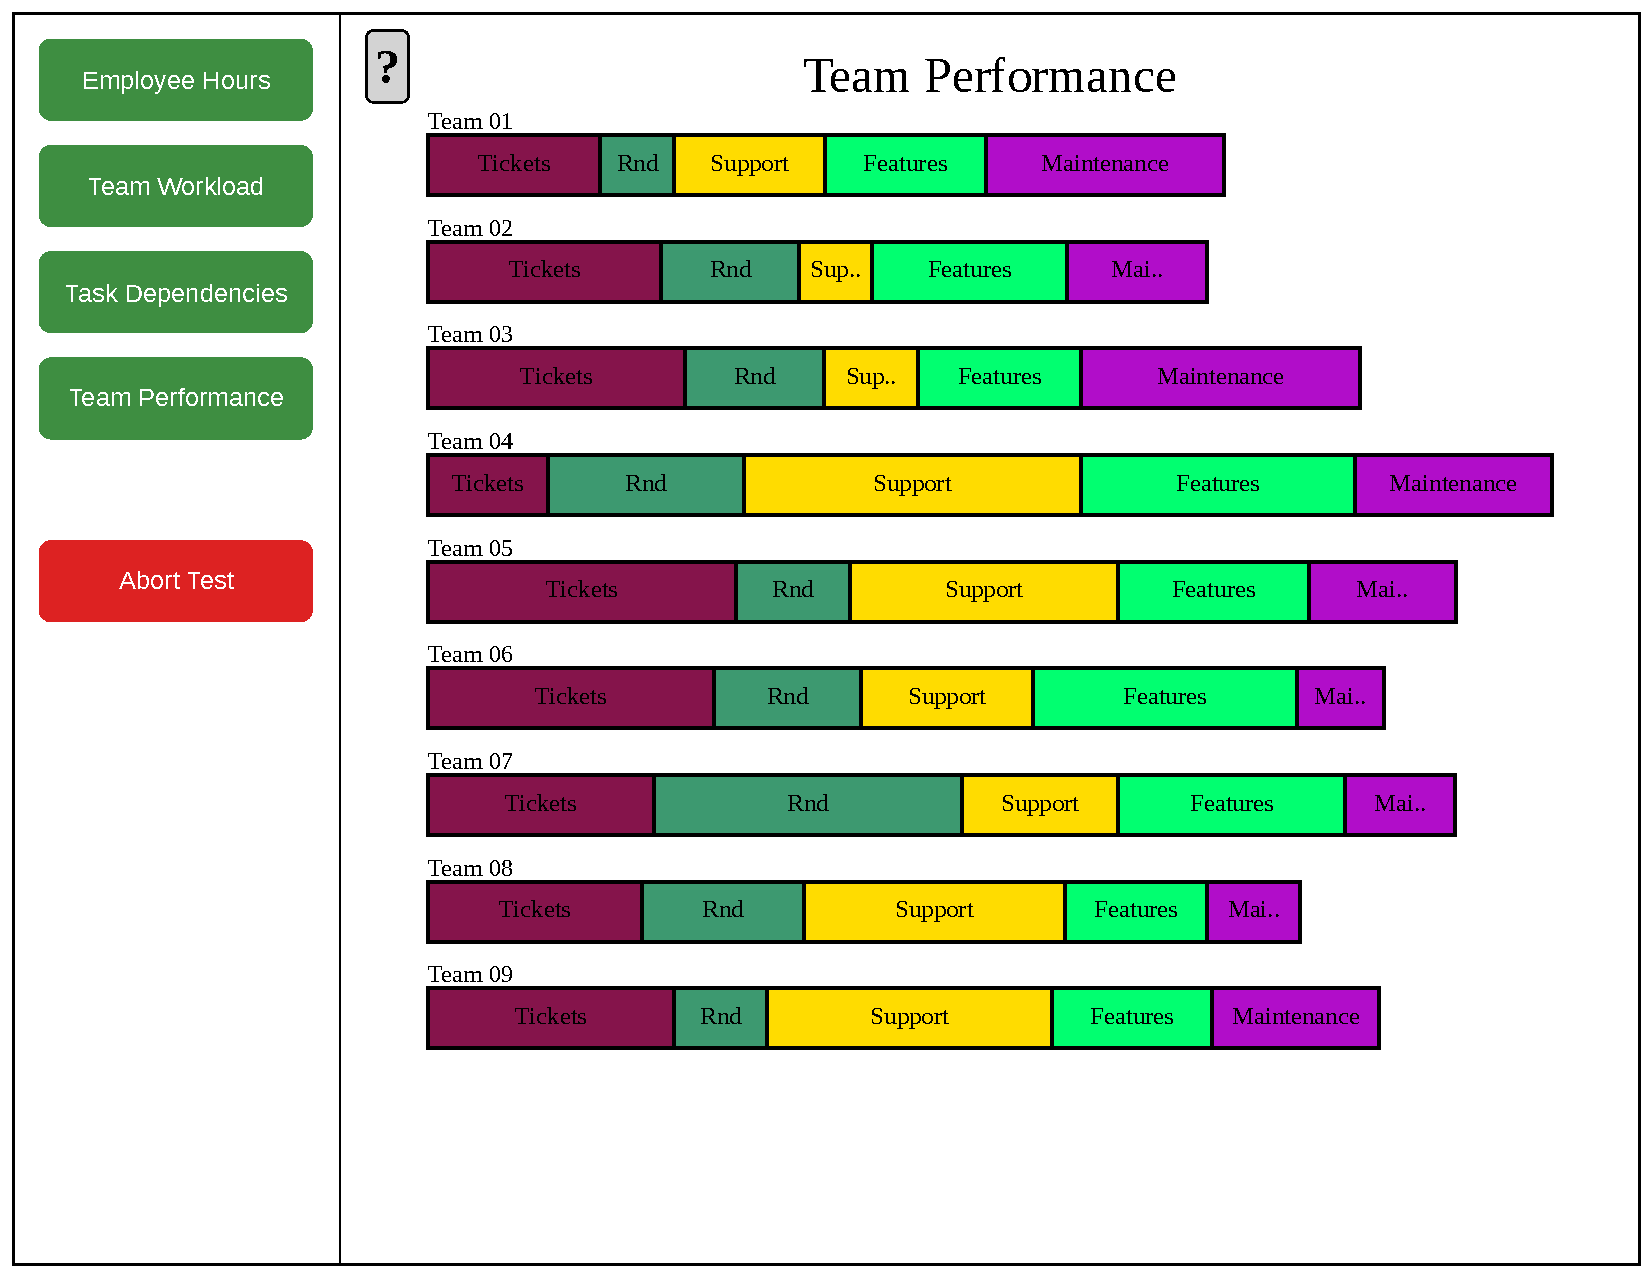
\includegraphics[width=.49\textwidth]{figures/captures/webapp_team_performance_task.pdf}
      \caption{Capture of Team Performance info- and task-page.}
    \end{figure}

		The goal for this tasks is to find which team did the most work,
		represented by having the longest bar, and additionally, click the largest
		segment, representing the type of task they got the work done on. As with
		the other tasks, this is timed, and faster is better.
